\RequirePackage{currfile}
\documentclass[12pt]{beamer}
\usepackage[utf8]{inputenc}
\usepackage[spanish]{babel}
\usepackage{standalone}
\usepackage{color}
\usepackage{siunitx}
\usepackage{hyperref}
%\hypersetup{colorlinks,linkcolor=,urlcolor=blue}
%\hypersetup{colorlinks,urlcolor=blue}
\usepackage{xcolor,soul}
\usepackage{etoolbox}
\usepackage{amsmath}
\usepackage{amsthm}
\usepackage{physics}
\usepackage{multicol}
\usepackage{bookmark}
\usepackage{longtable}
\usepackage{listings}
\usepackage{graphicx}
\usepackage{tikz}
\usetikzlibrary{patterns, matrix, backgrounds, decorations,shapes, arrows.meta}
\usepackage[autostyle,spanish=mexican]{csquotes}
\usepackage[os=win]{menukeys}
\usepackage{pifont}
\usepackage{pbox}
\usepackage{caption}
\captionsetup{font=scriptsize,labelfont=scriptsize}
%\usepackage[sfdefault]{roboto}  %% Option 'sfdefault' only if the base font of the document is to be sans serif

%Sección de definición de colores
\definecolor{ao}{rgb}{0.0, 0.5, 0.0}
\definecolor{bisque}{rgb}{1.0, 0.89, 0.77}
\definecolor{amber}{rgb}{1.0, 0.75, 0.0}
\definecolor{armygreen}{rgb}{0.29, 0.33, 0.13}
\definecolor{alizarin}{rgb}{0.82, 0.1, 0.26}
\definecolor{cadetblue}{rgb}{0.37, 0.62, 0.63}
\definecolor{deepblue}{rgb}{0,0,0.5}
\definecolor{brown}{rgb}{0.59, 0.29, 0.0}
\definecolor{OliveGreen}{rgb}{0,0.25,0}


\usefonttheme[onlymath]{serif}
%Sección de definición de nuevos comandos

\newcommand*{\TitleParbox}[1]{\parbox[c]{1.75cm}{\raggedright #1}}%
\newcommand{\python}{\texttt{python}}
\newcommand{\textoazul}[1]{\textcolor{blue}{#1}}
\newcommand{\azulfuerte}[1]{\textcolor{blue}{\textbf{#1}}}
\newcommand{\funcionazul}[1]{\textcolor{blue}{\textbf{\texttt{#1}}}}
\newcommand{\ptilde}[1]{\ensuremath{{#1}^{\prime}}}
\newcommand{\stilde}[1]{\ensuremath{{#1}^{\prime \prime}}}
\newcommand{\ttilde}[1]{\ensuremath{{#1}^{\prime \prime \prime}}}
\newcommand{\ntilde}[2]{\ensuremath{{#1}^{(#2)}}}
\renewcommand{\arraystretch}{1.5}

\newcounter{saveenumi}
\newcommand{\seti}{\setcounter{saveenumi}{\value{enumi}}}
\newcommand{\conti}{\setcounter{enumi}{\value{saveenumi}}}
\renewcommand{\rmdefault}{cmr}% cmr = Computer Modern Roman

\linespread{1.5}

\usefonttheme{professionalfonts}
%\usefonttheme{serif}
\DeclareGraphicsExtensions{.pdf,.png,.jpg}


%Sección para el tema de beamer, con el theme, usercolortheme y sección de footers
\mode<presentation>
{
  \usetheme{CambridgeUS}
  \setbeamertemplate{headline}{}
  %\useoutertheme{infolines}
  \useoutertheme{default}
  \usecolortheme{rose}
  \setbeamercovered{invisible}
  % or whatever (possibly just delete it)
  \setbeamertemplate{section in toc}[sections numbered]
  \setbeamertemplate{subsection in toc}[subsections numbered]
  \setbeamertemplate{subsection in toc}{\leavevmode\leftskip=3.2em\rlap{\hskip-2em\inserttocsectionnumber.\inserttocsubsectionnumber}\inserttocsubsection\par}
  \setbeamercolor{section in toc}{fg=blue}
  \setbeamercolor{subsection in toc}{fg=blue}
  \setbeamercolor{frametitle}{fg=blue}

  \setbeamertemplate{footline}
  %\beamertemplatenavigationsymbolsempty
}

\makeatletter
\setbeamercolor{section in foot}{bg=gray!30, fg=black!90!orange}
\setbeamercolor{subsection in foot}{bg=blue!30!yellow, fg=red}
\setbeamertemplate{footline}
{
  \leavevmode%
  \hbox{%
  \begin{beamercolorbox}[wd=.333333\paperwidth,ht=2.25ex,dp=1ex,center]{section in foot}%
    \usebeamerfont{section in foot} \insertsection
  \end{beamercolorbox}}%
  \begin{beamercolorbox}[wd=.333333\paperwidth,ht=2.25ex,dp=1ex,center]{subsection in foot}%
    \usebeamerfont{subsection in foot}  \insertsubsection
  \end{beamercolorbox}%
  \begin{beamercolorbox}[wd=.333333\paperwidth,ht=2.25ex,dp=1ex,right]{date in head/foot}%
    \usebeamerfont{date in head/foot} \insertshortdate{} \hspace*{2em}
    \insertframenumber{} / \inserttotalframenumber \hspace*{2ex} 
  \end{beamercolorbox}}%
  \vskip0pt%
\makeatother  

\makeatletter
\patchcmd{\beamer@sectionintoc}
  {\vfill}
  {\vskip\itemsep}
  {}
  {}
\makeatother

% \makeatletter
% \patchcmd{\hyper@link@}
%   {{\Hy@tempb}{#4}}
%   {{\Hy@tempb}{\ul{#4}}}
%   {}{}
% \makeatother


% Sección para el código

\definecolor{Code}{rgb}{0,0,0}
\definecolor{Keywords}{rgb}{255,0,0}
\definecolor{Strings}{rgb}{255,0,255}
\definecolor{Comments}{rgb}{0,0,255}
\definecolor{Numbers}{rgb}{255,128,0}

\DeclareCaptionFont{white}{\color{white}}
\DeclareCaptionFormat{listing}{\colorbox{gray}{\parbox{0.99\textwidth}{#1#2#3}}}
\captionsetup[lstlisting]{format=listing,labelfont=white,textfont=white}
\renewcommand{\lstlistingname}{Código}

\lstset{
basicstyle=\ttfamily,
columns=fullflexible,
breaklines=true
}

\lstdefinestyle{codigopython}{%
  language=Python,                % choose the language of the code
  %basicstyle=\footnotesize\small,       % the size of the fonts that are used for the code
  numbers=left,                   % where to put the line-numbers
  numberstyle=\scriptsize,      % the size of the fonts that are used for the line-numbers
  stepnumber=1,                   % the step between two line-numbers. If it is 1 each line will be numbered
  numbersep=5pt,                  % how far the line-numbers are from the code
  backgroundcolor=\color{white},  % choose the background color. You must add \usepackage{color}
  showspaces=false,               % show spaces adding particular underscores
  showstringspaces=false,         % underline spaces within strings
  showtabs=false,                 % show tabs within strings adding particular underscores
  frame=single,   		% adds a frame around the code
  tabsize=2,  		% sets default tabsize to 2 spaces
  captionpos=t,   		% sets the caption-position to bottom
  breaklines=true,    	% sets automatic line breaking
  breakatwhitespace=false,    % sets if automatic breaks should only happen at whitespace
  escapeinside={\#},  % if you want to add a comment within your code
  stringstyle =\color{OliveGreen},
  texcl = true,
  %otherkeywords={{as}},             % Add keywords here
  keywordstyle = \color{blue},
  commentstyle = \color{black},
  identifierstyle = \color{black},
  % literate=%
  %         {á}{{\'a}}1
  %         {é}{{\'e}}1
  %         {í}{{\'i}}1
  %         {ó}{{\'o}}1
  %         {ú}{{\'u}}1
  %
  %keywordstyle=\ttb\color{deepblue}
  %fancyvrb = true,
literate={0}{{\textcolor{red}{0}}}{1}%
            {1}{{\textcolor{red}{1}}}{1}%
            {2}{{\textcolor{red}{2}}}{1}%
            {3}{{\textcolor{red}{3}}}{1}%
            {4}{{\textcolor{red}{4}}}{1}%
            {5}{{\textcolor{red}{5}}}{1}%
            {6}{{\textcolor{red}{6}}}{1}%
            {7}{{\textcolor{red}{7}}}{1}%
            {8}{{\textcolor{red}{8}}}{1}%
            {9}{{\textcolor{red}{9}}}{1}%
            {.0}{{\textcolor{red}{.0}}}{2}% Following is to ensure that only periods
            {.1}{{\textcolor{red}{.1}}}{2}% followed by a digit are changed.
            {.2}{{\textcolor{red}{.2}}}{2}%
            {.3}{{\textcolor{red}{.3}}}{2}%
            {.4}{{\textcolor{red}{.4}}}{2}%
            {.5}{{\textcolor{red}{.5}}}{2}%
            {.6}{{\textcolor{red}{.6}}}{2}%
            {.7}{{\textcolor{red}{.7}}}{2}%
            {.8}{{\textcolor{red}{.8}}}{2}%
            {.9}{{\textcolor{red}{.9}}}{2}%
            {\ }{{ }}{1}% handle the space
        ,%
        %mathescape=true
        %escapeinside={*@}
        escapeinside={A_}{_B}
}

%\newcommand\numberthis{\addtocounter{equation}{1}\tag{\theequation}}
\title{Tema 3 - Ecuaciones diferenciales ordinarias}
\subtitle{Curso de Física Computacional}
\author[]{M. en C. Gustavo Contreras Mayén}
\date{15 de abril de 2020}
\begin{document}
\maketitle
\fontsize{14}{14}\selectfont
\spanishdecimal{.}
\section*{Contenido}
\frame[allowframebreaks]{\tableofcontents[currentsection, hideallsubsections]}
\section{Introducción}
\frame{\tableofcontents[currentsection, hideothersubsections]}
\subsection{Motivación}
\begin{frame}
\frametitle{Introducción}
La importancia particular de los métodos numéricos para resolver ecuaciones diferenciales ordinarias (EDO) o sus sistemas se debe al hecho de que muchas de las leyes de la naturaleza se expresan convenientemente en forma diferencial.
\end{frame}
\begin{frame}
\frametitle{Introducción}
Las ecuaciones clásicas de movimiento de partículas, las ecuaciones de difusión de masa o transporte de calor, o la ecuación de onda de Schrödinger son solo algunos ejemplos que ilustran la extraordinaria diversidad de fenómenos físicos esencialmente diferentes, que se modelan mediante ecuaciones diferenciales.
\end{frame}
\begin{frame}
\frametitle{Introducción}
Una multitud de fenómenos se describen mediante ecuaciones diferenciales parciales (EDP), lo que implica derivadas de varios órdenes de la función desconocida con respecto a varias variables independientes.
\end{frame}
\begin{frame}
\frametitle{Introducción}
Nuevamente, en muchas situaciones, uno tiene que lidiar con las EDO dependiendo de las derivadas de varios órdenes de la función desconocida con respecto a una sola variable independiente.
\end{frame}
\begin{frame}
\frametitle{Introducción}
Las EDO pueden ser intrínsecamente ordinarias, es decir, pueden resultar como tales del modelado mismo del fenómeno en cuestión, o pueden resultar de un proceso previo de separación de variables de una EDP inicial, generalmente aprovechando ciertas propiedades de simetría presentadas por el sistema modelado.
\end{frame}
\begin{frame}
\frametitle{Introducción}
En una situación más compleja, la solución puede comprender varias funciones desconocidas, que satisfacen un sistema de EDO acopladas.
\end{frame}
\begin{frame}
\frametitle{Conexión en una EDO y un sistema de EDO}
Como ejemplo que muestra la conexión cerca entre EDO de orden superior y sistemas de EDO, consideremos el ejemplo clásico de la primera ley de Newton, que expresa la ecuación de movimiento de una partícula de masa $m$, experimentando una fuerza $F(x)$:
\begin{align}
m \, \dv[2]{x}{t} =  F(x)
\label{eq:ecuacion_12_01}
\end{align}
\end{frame}
\begin{frame}
\frametitle{Ejemplo de la mecánica}
Definiendo el momento de la partícula como $p = m \, (\dv*{x}{t})$, que es una EDO2 que puede descomponerse en un conjunto de dos ecuaciones diferenciales de primer orden:
\begin{align}
\dv{x}{t} = \dfrac{p}{m}, \hspace{0.5cm} \dv{p}{t} = F(x)
\label{eq:ecuacion_12_02}
\end{align}
que son las llamadas \emph{ecuaciones canónicas de Hamilton del movimiento}.
\end{frame}
\begin{frame}
\frametitle{Ejemplo de la mecánica}
Enfatizando en la velocidad de la partícula $v=p/m$ que su momento, las ecuaciones anteriores se vuelven
\begin{align}
\dv{x}{t} = v \hspace{0.5cm} \dv{v}{t} = \dfrac{1}{m} \, F(x)
\label{eq:ecuacion_12_03}
\end{align}
\end{frame}
\begin{frame}
\frametitle{Ejemplo de la mecánica}
Mediante la forma funcional equivalente de las EDO1 que componen este sistema acoplado, las dos funciones desconocidas, $x$ y $v$, se establecen en igualdad de condiciones.
\end{frame}
\begin{frame}
\frametitle{Ejemplo de la mecánica}
Además, la metodología de transformar la ecuación de movimiento inicial (\ref{eq:ecuacion_12_01}) en un sistema (\ref{eq:ecuacion_12_03}) revela que, en principio, es suficiente desarrollar solo métodos para resolver EDO1 o sistemas de tales ecuaciones.
\end{frame}
\begin{frame}
\frametitle{Alcance del Tema 3}
Sin embargo, debido a la importancia práctica particular de las ecuaciones de movimiento de segundo orden (por ejemplo en la dinámica molecular cuántica o clásica), se desarrollarán métodos numéricos específicos para resolver EDO o sistemas de segundo orden.
\end{frame}
\section{Ecuaciones Diferenciales Ordinarias}
\frame{\tableofcontents[currentsection, hideothersubsections]}
\subsection{Notación para las EDO}
\begin{frame}
\frametitle{Notación para las EDO}
Consideremos una ecuacion diferencial de orden $n$ (EDOn) para la función desconocida $y(t)$:
\begin{align}
\ntilde{y}{n} = f(t, y, \ptilde{y}, \ldots, \ntilde{y}{n-1})
\label{eq:ecuacion_12_04}
\end{align}
\end{frame}
\begin{frame}
\frametitle{Reducción de orden de la EDO}
Se puede demostrar fácilmente que la ecuación anterior, es equivalente a un sistema de $n$ EDO1:
\begin{align}
\ptilde{y}_{i} (t) = f_{i} (y, y_{1} (t), y_{2} (t), \ldots, y_{n} (t) ) \hspace{0.5cm} i = 1, 2, \ldots, n
\label{eq:ecuacion_12_05}
\end{align}
\end{frame}
\begin{frame}
\frametitle{Reducción de orden de las EDO}
Al considerar como funciones desconocidas además de $y$, también sus primeras $(n-1)$ derivadas
\begin{align*}
y_{i} \equiv \ntilde{y}{i-1}, \hspace{0.5cm} i = 1, 2, \ldots, n
\end{align*}
identificando la incógnita original con la primera de las nuevas funciones desconocidas, $y \equiv y_{1}$
\end{frame}
\begin{frame}
\frametitle{Nuevo sistema de ecuaciones}
Entonces el sistema que se obtiene, es de la forma:
\begin{align*}
\begin{cases}
\ptilde{y}_{i} (t) = y_{i+1} (t), \hspace{1cm} i = 1, 2, \ldots, n-1 \\
\ptilde{y}_{n} (t) = f(t, y_{1} (t), y_{2} (t), \ldots, y_{n} (t))
\end{cases}
\end{align*}
\end{frame}
\begin{frame}
\frametitle{Nuevo sistema de ecuaciones}
Donde las primeras $(n - 1$ ecuaciones resultan de notaciones simples y no son específicas, mientras que solo la última ecuación contiene la función particular del lado derecho $f$, que es específica del problema.
\end{frame}
\subsection*{Notación simplificada}
\begin{frame}
\frametitle{Notación simplificada}
Para simplificar la notación para el desarrollo de los métodos de solución numérica, el sistema general de EDO1 (ec. \ref{eq:ecuacion_12_05}), se puede escribir con una notación vectorial:
\begin{align}
\ptilde{y} (t) = f (t, y)
\label{eq:ecuacion_12_06}
\end{align}
\end{frame}
\begin{frame}
\frametitle{Notación simplificada}
Donde
\begin{align*}
y = \begin{bmatrix}
y_{1} (t) \\
\vdots \\
y_{n} (t)
\end{bmatrix}
\hspace{1.5cm}
f(t, y) =
\begin{bmatrix}
f_{1} (t, y_{1} (t), \ldots, y_{n} (t)) \\
\vdots \\
f_{n} (t, y_{1} (t), \ldots, y_{n} (t))
\end{bmatrix}
\end{align*}
\end{frame}
\begin{frame}
\subsection*{Alcance del análisis}
\frametitle{Alcance del análisis}
En las siguientes diapositivas no se discuten explícitamente los métodos para resolver sistemas de EDO, ya que estos pueden obtenerse simplemente de aquellos para ecuaciones individuales, reemplazando el escalar con anotaciones vectoriales.
\end{frame}
\subsection*{Condiciones para la solución}
\begin{frame}
\frametitle{Condiciones para la solución}
Un problema para una EDO es que no está completamente especificada únicamente por la ecuación misma.
\\
\bigskip
\pause
Para obtener una solución particular de la familia de soluciones compatibles, uno debe adjuntar condiciones adicionales relativas a los valores de la solución en ciertos puntos del dominio de definición.
\end{frame}
\begin{frame}
\frametitle{Condiciones para la solución}
Más que por la forma específica de la EDO, el tipo de estrategia numérica que es adecuada para resolver el problema está determinado por estas condiciones adicionales.
\end{frame}
\begin{frame}
\frametitle{Tipos de condiciones para la solución}
Esencialmente, las condiciones adicionales que se pueden asociar a las EDO se dividen en dos grandes categorías:
\setbeamercolor{item projected}{bg=blue!70!black,fg=yellow}
\setbeamertemplate{enumerate items}[circle]
\begin{enumerate}[<+->]
\item Problemas de valores iniciales (\emph{de Cauchy}).
\item Problemas con dos puntos como condiciones de frontera (\emph{CDF bilocales}).
\end{enumerate}
\end{frame}
\section{Problemas de valores iniciales}
\frame{\tableofcontents[currentsection, hideothersubsections]}
\subsection{Definición del problema}
\begin{frame}
\frametitle{Definición del problema}
Un problema de valores iniciales se obtiene al agregar al sistema (ec. \ref{eq:ecuacion_12_06}), las $n$ condiciones adicionales en el punto inicial $t_{0}$.
\begin{align}
y_{i} (t_{0}) = y_{i0} \hspace{1.5cm} i = 1, 2, \ldots, n
\label{eq:ecuacion_12_07}
\end{align}
\pause
O en notación vectorial
\begin{align}
y(t_{0}) = y_{0}
\label{eq:ecuacion_12_08}
\end{align}
\end{frame}
\subsection*{Solución al problema}
\begin{frame}
\frametitle{Solución al problema}
Resolver este problema implica el cálculo progresivo, paso a paso, de la solución en una secuencia de puntos $t_{0}, t_{1}, t_{2}, \ldots$
\end{frame}
\begin{frame}
\frametitle{Solución al problema}
Los problemas de valores iniciales generalmente dependen, aunque no siempre, del tiempo como una variable independiente y describen la evolución del sistema modelado.
\end{frame}
\begin{frame}
\frametitle{Solución al problema}
Un ejemplo típico es el lanzamiento inclinado de un proyectil que experimenta gravitación y arrastre.
\\
\bigskip
Las ecuaciones de movimiento de Newton únicamente proporcionan una familia de soluciones parametrizadas con constantes de integración arbitrarias. 
\end{frame}
\begin{frame}
\frametitle{Solución al problema}
Sin embargo, una solución particular, que describe una situación física concreta, solo puede obtenerse especificando también valores iniciales para los vectores de posición y velocidad del proyectil.
\end{frame}
\subsection*{Tipos de solución}
\begin{frame}
\frametitle{Tipos de solución}
A su vez, los métodos para resolver problemas de valores iniciales se pueden dividir en dos clases. 
\setbeamercolor{item projected}{bg=blue!70!black,fg=yellow}
\setbeamertemplate{enumerate items}[circle]
\begin{enumerate}[<+->]
\item Los \emph{métodos directos} o de un sólo paso.
\item Los \emph{métodos indirectos} o de varios pasos.
\end{enumerate}
\end{frame}
\subsection*{Métodos directos}
\begin{frame}
\frametitle{Métodos directos}
La primera clase comprende los llamados \textoazul{métodos directos} o de un solo paso, que proporcionan la solución en algún punto $t_{m+1}$ basado únicamente en información (solución y derivadas) del punto anterior, $t_{m}$ y, posiblemente, del intervalo $[t_{m} , t_{m + 1}]$.
\end{frame}
\begin{frame}
\frametitle{Métodos directos}
El número de condiciones iniciales asociadas tiene que coincidir para con el orden de la EDO, mientras que para un sistema de EDO, con el orden acumulado de las ecuaciones involucradas.
\end{frame}
\subsection*{Algunos métodos directos}
\begin{frame}
\frametitle{Algunos de métodos directos}
Mencionamos de esta categoría los métodos generales de \textoazul{Euler} y \textoazul{Runge-Kutta}, así como los métodos más adaptados: de \textoazul{Euler-Cromer}, \textoazul{Euler-Richardson} y \textoazul{Verlet}.
\end{frame}
\subsection*{Métodos indirectos}
\begin{frame}
\frametitle{Métodos indirectos}
La segunda clase de algoritmos para problemas de valores iniciales reúne los llamados \textoazul{métodos indirectos} o de varios pasos, que permiten el cálculo de la solución en algún punto $t_{m+1}$ en función de la información de varios puntos anteriores $t_{m}, t_{m-1}, \ldots$.
\end{frame}
\subsection*{Algunos métodos indirectos}
\begin{frame}
\frametitle{Algunos de métodos indirectos}
De esta categoría, mencionamos los métodos \textoazul{Adams-Moulton}, \textoazul{Milne}, \textoazul{Fox-Goodwin} y \textoazul{Numerov}.
\end{frame}
\subsection*{Consideraciones de ambos métodos}
\begin{frame}
\frametitle{Consideraciones de ambos métodos}
Los métodos de cada una de las dos clases presentan ventajas y desventajas específicas, siendo típicamente efectivos bajo diferentes circunstancias y sujetos a diferentes requisitos.
\\
\bigskip
Por lo que se debe de tener cuidado al inicio del planteamiento del problema a estudiar,
\end{frame}
\section{Problemas con CDF de dos puntos}
\frame{\tableofcontents[currentsection, hideothersubsections]}
\subsection{Definición del problema}
\begin{frame}
\frametitle{Definición del problema}
Al asociar a una EDO con condiciones adicionales con respecto a la solución y, posiblemente, sus derivadas en los extremos del rango de definición $[x_{1}, x_{2}]$:
\begin{align}
\alpha_{1} \, y(x_{1}) + \beta_{1} \, \ptilde{y} (x_{1}) &= \gamma_{1} \label{eq:ecuacion_12_09} \\[0.5em]
\alpha_{2} \, y(x_{2}) + \beta_{2} \, \ptilde{y} (x_{2}) &= \gamma_{2} \label{eq:ecuacion_12_10}
\end{align}
que es el llamado \emph{problema de dos puntos}.
\end{frame}
\subsection*{Solución al problema}
\begin{frame}
\frametitle{Solución al problema}
Como en el caso de los problemas de Cauchy, el número de condiciones adicionales tiene que coincidir, aquí también, con los órdenes acumulados de las ecuaciones.
\\
\bigskip
El objetivo de cualquier enfoque numérico es en este caso, el cálculo de la solución en algunos puntos de malla interiores del dominio $[x_{1}, x_{2}]$.
\end{frame}
\begin{frame}
\frametitle{Ejemplos de problemas}
Los típicos problemas físicos que se pueden modelar como problemas de dos puntos se refieren a la deformación de una cuerda sujeta o una viga soportada.
\\
\bigskip
Revisaremos el \textoazul{método de disparo} y el \textoazul{método de diferencias finitas}  para resolver los problemas bilocales asociados a las EDO lineales de segundo orden.
\end{frame}
\section{Técnicas directas de solución}
\frame[allowframebreaks]{\tableofcontents[currentsection, hideothersubsections]}
\subsection{Método de la serie de Taylor}
\begin{frame}
\frametitle{Método de la serie de Taylor}
Uno de los métodos más antiguos y generales para resolver problemas de valores iniciales para una EDO se basa en la expansión de la solución en una serie de Taylor.
\\
\bigskip
\emph{El método de la serie Taylor} permite, en principio, la solución de cualquier ecuación diferencial, pero su aplicación práctica es a menudo difícil e ineficiente.
\end{frame}
\begin{frame}
\frametitle{Método de la serie de Taylor}
La importancia de este método reside más bien en su capacidad para proporcionar criterios para evaluar la precisión de los métodos de interés práctico.
\\
\bigskip
Básicamente, la idea subyacente es reemplazar las diferenciaciones por operaciones de diferencias finitas.
\end{frame}
\begin{frame}
\frametitle{Método de la serie de Taylor}
Consideremos el problema de valores iniciales:
\begin{align}
\ptilde{y} &= f(t, y) \label{eq:ecuacion_12_11} \\
y(t_{0}) &= y_{0} \label{eq:ecuacion_12_12}
\end{align}
\end{frame}
\begin{frame}
\frametitle{Método de la serie de Taylor}
Suponemos que existe una solución, que es: única, finita y expandible en una serie de Taylor en la vecindad del punto inicial $t_{0}$
\begin{align}
y(t) = y_(t_{0}) + \dfrac{t - t_{0}}{1!} \, \ptilde{y} (t_{0}) + \dfrac{(t - t_{0}^{2})}{2!} \, \stilde{y} (t_{0}) + \ldots
\label{eq:ecuacion_12_13}
\end{align}
\end{frame}
\begin{frame}
\frametitle{Método de la serie de Taylor}
La expansión de Taylor (ec. \ref{eq:ecuacion_12_13}) proporciona un procedimiento \emph{paso a paso} para evaluar la solución $y (t)$ en los puntos de la malla dados por $t_{0}, t_{1}, \ldots, t_{m}, \ldots$ como una secuencia de soluciones de problemas elementales de Cauchy.
\end{frame}
\begin{frame}
\frametitle{Método de la serie de Taylor}
Específicamente, propagar la solución de $t_{m}$ a $t_{m + 1}$ es equivalente a resolver la ecuación diferencial (\ref{eq:ecuacion_12_11}) sujeta a la condición inicial
\begin{align*}
y(t_{m}) = y_{m}
\end{align*}
y se logra en base a la expansión:
\end{frame}
\begin{frame}
\frametitle{Método de la serie de Taylor}
La expansión es
\begin{align}
y_{m+1} = y_{m} + h \, \ptilde{y}_{m} + \dfrac{h^{2}}{2} \, \stilde{y}_{m} + \ldots
\label{eq:ecuacion_12_14}
\end{align}
donde $y \equiv y(t_{m})$, $\ptilde{y}_{m} \equiv \ptilde{y} (t_{m})$, $\stilde{y}_{m} \equiv \stilde{y}_{m}$ 
\end{frame}
\begin{frame}
\frametitle{Método de la serie de Taylor}
El espaciamiento en la malla está dado por
\begin{align*}
h = t_{m+1} - t-{m}
\end{align*}
Cuanto más pequeño sea el espaciado de malla $h$ en comparación con el radio de convergencia de la serie, y cuanto mayor sea el número de términos mantenidos en serie (ec. \ref{eq:ecuacion_12_14}), más cercana será la estimación $y_{m + 1}$ a la solución exacta $y(t_{m + 1})$.
\end{frame}
\begin{frame}
\frametitle{Método de la serie de Taylor}
La estimación de la solución propagada $y_{m + 1}$ requiere las derivadas en $t_{m}$, llamadas $\ptilde{y}_{m}, \stilde{y}_{m}, \ldots$
\\
\bigskip
De hecho, la primera derivada ya está disponible desde la propia EDO (\ref{eq:ecuacion_12_11}) y solo necesita ser evaluada en $t_{m}$:
\begin{align*}
\ptilde{y}_{m} = f( t_{m}, y_{m})
\end{align*}
\end{frame}
\begin{frame}
\frametitle{Método de la serie de Taylor}
Por otro lado, al tomar las derivadas de ambos miembros de la ec. \ref{eq:ecuacion_12_11} con respecto a $t$ (teniendo en cuenta que $f$ es una función de $t$ tanto explícitamente como a través de $y$), se encuentra la segunda derivada en $t_{m}$:
\begin{align*}
\stilde{y}_{m} = \left[ \pdv{f}{t} + \pdv{f}{y} \, \pdv{y}{t} \right]_{t_{m}, y_{m}} = \left[ \pdv{f}{t} + f \, \pdv{f}{y} \right]_{t_{m}, y_{m}}
\end{align*}
\end{frame}
\begin{frame}
\frametitle{Método de la serie de Taylor}
Al incorporar las expresiones de $\ptilde{y}_{m}$ y $\stilde{y}_{m}$ en la expansión de la ec. \ref{eq:ecuacion_12_14}), tenemos la relación de propagación:
\begin{align}
\begin{aligned}
y_{m+1} &= y_{m} + h \, f(t_{m}, y_{m}) + \\
&+ \dfrac{h^{2}}{2} \left[\pdv{f}{t} + f \, \pdv{f}{y} \right]_{t_{m}, y_{m}} + \order{h^{3}}
\end{aligned}
\label{eq:ecuacion_12_15}
\end{align}
\end{frame}
\begin{frame}
\frametitle{Método de la serie de Taylor}
La notación $\order{h^{3}}$ indica que el error de truncamiento es del orden $h^{3}$, es decir, todos los términos que no se consideran, implican $h$ con potencias mayores o iguales a tres, mientras que los términos que permanecen, implican como máximo $h^{2}$.
\end{frame}
\begin{frame}
\frametitle{Método de la serie de Taylor}
El método de la serie de Taylor es claramente un \emph{método de un solo paso}, ya que para calcular $y_{m+1}$, se necesita nada más la información del punto precedente $t_{m}$.
\end{frame}
\begin{frame}
\frametitle{Desventajas del método}
Para aproximaciones de orden superior de la solución, uno debe considerar términos adicionales en la serie (ec. \ref{eq:ecuacion_12_14}).
\\
\bigskip
De todos modos, las derivadas implícitas de orden superior se vuelven cada vez más complejas, tanto para derivar como para programar, lo que lleva a fórmulas de propagación ineficientes. En ciertas situaciones, la evaluación de los derivadas se vuelve imposible.
\end{frame}
\begin{frame}
\frametitle{Relevancia del método}
A pesar de las deficiencias prácticas, el método de la serie Taylor conserva, como ya se mencionó, una importancia teórica especial, ya que proporciona un criterio unificador para evaluar la precisión de otros métodos para los problemas de Cauchy.
\end{frame}
\begin{frame}
\frametitle{Criterio unificador del método}
El criterio se refiere al grado en que la solución aproximada coincide con la expansión de la serie Taylor de la solución exacta.
\\
\bigskip
\pause
Más precisamente, se dice que un método es de orden $p$ si la solución aproximada es equivalente a la serie de Taylor exacta hasta los términos del orden $h^{p}$, o, de manera equivalente, si el error de truncamiento del método es $\order{h^{p+1}}$.
\end{frame}
\begin{frame}
\frametitle{Criterio unificador del método}
Esta forma de evaluar la clase de precisión también sigue siendo aplicable a los métodos que ni siquiera implican la evaluación efectiva de las derivadas de la función del lado derecho $f(t, y)$ de la EDO.
\end{frame}
\subsection{Método de Euler}
\begin{frame}
\frametitle{El método de Euler}
\emph{El método de Euler}, también llamado \emph{Euler directo} o \emph{método explícito de Euler}, es el método más simple de un solo paso para problemas de valores iniciales.
\end{frame}
\begin{frame}
\frametitle{El método de Euler}
Refiriéndose nuevamente al problema general de Cauchy ecs. \ref{eq:ecuacion_12_11}-\ref{eq:ecuacion_12_12}, el método de Euler es simplemente la aproximación lineal del método de la serie de Taylor con los términos menores a $\order{h^{2}}$:
\begin{align}
y_{m+1} =  y_{m} +  h \, f(t_{m}, y_{m}) \hspace{1cm} m = 0, 1, 2, \ldots
\label{eq:ecuacion_12_16}
\end{align}
con $h = t_{m+1} - t_{m}$
\end{frame}
\begin{frame}
\frametitle{Método de Euler}
Señalamos nuevamente el hecho de que $y_{m}$ puede representar aquí un solo valor (en el caso de una sola EDO), o puede representar un vector de componentes de la solución (en el caso de un sistema de EDO).
\end{frame}
\begin{frame}
\frametitle{Relación de recurrencia}
La relación de recurrencia (\ref{eq:ecuacion_12_16}) proporciona explícitamente la solución propagada $y_{m + 1}$ en términos del valor anterior $y_{m}$ (considerado como valor inicial de un problema de Cauchy elemental).
\\
\bigskip
Por lo tanto, a partir de un valor inicial $y_{0} = y(t_{0})$, se puede determinar, paso a paso, la secuencia de aproximaciones $y_{1}, y_{2}, \ldots,$ de los valores exactos de la solución $y(t_{1}), y(t_{2}), \ldots$
\end{frame}
\begin{frame}
\frametitle{Descripción gráfica del método}
La figura (\ref{fig:figura_12_01}) muestra que la aplicación repetida del método de Euler equivale a reemplazar la curva $y = y (t)$ con la función lineal por partes que conecta los puntos $(t_{0}, y_{0}), (t_{1}, y_{1}), (t_{2}, y_{2}), \ldots$.
\end{frame}
\begin{frame}
\frametitle{Descripción gráfica del método}
\begin{figure}[h!]
    \centering
    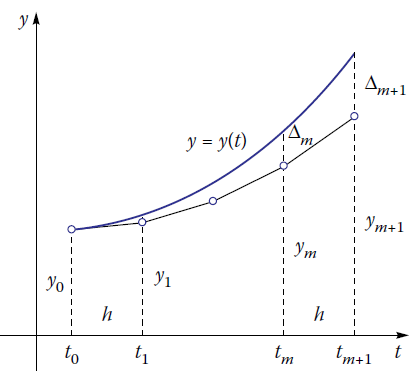
\includegraphics[scale=0.5]{Imagenes/metodoEuler_01.png}
    \caption{Las soluciones aproximadas $y_{m + 1}$ propagadas por el método de Euler se encuentran en las líneas tangentes a las soluciones exactas de la EDO que pasa a través de $(x_{m}, y_{m})$, $m = 0, 1, 2, \ldots$}
    \label{fig:figura_12_01}
\end{figure}
\end{frame}
\begin{frame}
\frametitle{Descripción gráfica del método}
El segmento inicial representa la línea tangente a la solución exacta que pasa por el punto inicial $(t_{0}, y_{0})$.
\\
\bigskip
En general, la solución propagada $y_{m + 1}$ puede considerarse como la extrapolación en línea recta de la solución particular de la EDO que pasa por el punto anterior $(t_{m}, y_{m})$, sin embargo, no necesariamente satisface la condición inicial $y(t_{0}) = ( y_{0})$.
\end{frame}
\begin{frame}
\frametitle{Error local del método}
El método de Euler es un algoritmo con error del tipo $\order{h}$, ya que la solución propagada coincide con la serie de Taylor en términos proporcionales a $h$.
\\
\bigskip
El error local está dominado por el error de truncamiento $\order{h^{2}}$ y caracteriza la desviación de $y_{m + 1}$ de la solución particular que pasa por $(t_{m}, y_{m})$.
\end{frame}
\begin{frame}
\frametitle{Error global del método}
El error global acumula los errores locales a lo largo de la propagación y mide la desviación total $\Delta_{m+ 1} = y_{m + 1} - y(t_{m + 1})$ de la solución aproximada $y_{m + 1}$ de la solución exacta.
\end{frame}
\begin{frame}
\frametitle{Error global del método}
El error global obviamente aumenta con el número de pasos de propagación y, según un teorema de convergencia general, si el error local de un método de solución de la EDO de un paso es $\order{h^{p + 1}}$, entonces el error global es $\order{h^{p}}$.
\\
\bigskip
\pause  
El error de truncamiento global del método de Euler es, por lo tanto, $\order{h}$.
\end{frame}
\begin{frame}
\frametitle{Consideraciones sobre el valor de $h$}
En este punto, es importante subrayar que disminuir de manera indefinida el tamaño del paso $h$ de cualquier procedimiento para resolver una EDO, con el objetivo de reducir el error de truncamiento y obtener en el límite la solución \enquote{exacta}, no es un enfoque práctico.
\end{frame}
\begin{frame}
\frametitle{Consideraciones sobre el valor de $h$}
De hecho, la acumulación de errores de redondeo, provocada por el aumento inherente del número de pasos de propagación, comienza a dominar la solución, que deja de mejorar por la reducción adicional de $h$ por debajo de un cierto valor.
\end{frame}
\subsection{Método predictor-corrector de Euler}
\begin{frame}
\frametitle{Método predictor-corrrector de Euler}
Una forma práctica de superar la baja precisión del método de Euler es \emph{elevar el orden de la aproximación} aplicando su variante llamada \textoazul{método de Euler predictor-corrector}.\end{frame}
\begin{frame}
\frametitle{Método predictor-corrector de Euler}
Este método opera con dos estimaciones de solución en cada paso de propagación:
\begin{align}
\tilde{y}_{m+1} &= y_{m} + h \, f(t_{m}, y_{m}) \hspace{1cm} m = 0, 1, 2, \ldots \label{eq:ecuacion_12_17} \\
y_{m+1} &= y_{m} + \dfrac{h}{2} \, \left[ f(t_{m}, y_{m}) + f(t_{m} + h \, \tilde{y}_{m+1}) \right] \label{eq:ecuacion_12_18}
\end{align}
\end{frame}
\begin{frame}
\frametitle{Familia de predictores-correctores}
Más adelante veremos que tanto los métodos básicos como los predictores-correctores de Euler se muestran como casos particulares de una familia completa de algoritmos, conocidos como \textoazul{métodos Runge-Kutta}.
\end{frame}
\begin{frame}
\frametitle{Familia de predictores-correctores}
El método básico de Euler es equivalente al \textoazul{método Runge-Kutta de primer orden (RK1)}.
\\
\bigskip
Mientras que el algoritmo de Euler predictor-corrector es $\order{h^{2}}$, es equivalente al \textoazul{método Runge-Kutta de segundo orden (RK2)}.
\end{frame}
\begin{frame}
\frametitle{Familia de predictores-correctores}
La precisión superior del algoritmo de Euler predictor-corrector obviamente se produce a expensas de un doble número de evaluaciones de las funciones del lado derecho $f(x, y)$ de las EDO.
\end{frame}
\begin{frame}
\frametitle{Algoritmo para los métodos}
El método Euler en sus variantes básica y predictor-corrector se propone en las funciones \funcionazul{Euler} y \funcionazul{EulerPC}, respectivamente.
\end{frame}
\begin{frame}
\frametitle{Crear un módulo para los algoritmos}
Es buen momento para crear un módulo con las funciones de los métodos directos de solución, que llamaremos \funcionazul{metodosdirectos.py}
\\
\bigskip
De esta manera tendremos localizados los códigos para los ejercicios y problemas.
\end{frame}
\begin{frame}
\frametitle{Argumentos para \funcionazul{Euler}}
La función propaga la solución $y$ de un sistema de EDO1:
\begin{align*}
\ptilde{y}[i] =  f[i] (t, y[]), \hspace{1cm} i = 1, 2, \ldots
\end{align*}
de $t$ a $t + h \, t$ mediante el método de Euler.
\\
\bigskip
Requiere la función \funcionazul{Func(t, y, f)}, que corresponde al lado derecho de la EDO.
\end{frame}
\begin{frame}[fragile]
\frametitle{Código propuesto \funcionazul{Euler}}
\begin{lstlisting}[caption=Código para el método de Euler, style=codigopython]
def Euler(t, ht, y, n, Func):
    f = [0]*(n+1)
 
    Func(t, y, f)
    for i in range(1, n+1): y[i] += ht * f[i]
\end{lstlisting}
\end{frame}
\begin{frame}[fragile]
\frametitle{Argumentos para la función \funcionazul{EulerPC}}
Propaga la solución $y$ de un sistema de EDO1:
\begin{align*}
\ptilde{y}[i] =  f[i] (t, y[]), \hspace{1cm} i = 1, 2, \ldots
\end{align*}
de $t$ a $t + h \, t$ mediante el método predictor-corrector de Euler.
\\
\bigskip
Requiere la función \funcionazul{Func(t, y, f)}, que corresponde al lado derecho de la EDO.
\end{frame}
\begin{frame}[allowframebreaks, fragile]
\frametitle{Código para \funcionazul{EulerPC}}
\begin{lstlisting}[caption=Código para el método predictor-corrector de Euler, style=codigopython]
def EulerPC(t, ht, y, n, Func):
    fA_1_B = [0]*(n+1); fA_2_B = [0]*(n+1)
    yt = [0]*(n+1)
 
    Func(t, y, f1)
    for i in range(1, n+1): yt[i] = y[i] + ht * fA_1_B[i]
    Func(t+ht, yt, fA_2_B)
 
    htA_2_B = ht/2e0
    for i in range(1, n+1): y[i] += htA_2_B * (fA_1_B[i] + fA_2_B[i]) 
\end{lstlisting}
\end{frame}
\begin{frame}
\frametitle{Ejemplo práctico}
Para revisar la precisión y la estabilidad de los métodos de Euler mencionados, consideremos un problema de tipo Cauchy para una EDO2 lineal:
\begin{align}
&\stilde{y} + y = 0 \label{eq:ecuacion_12_19} \\
&y(0) = y_{0}, \hspace{0.5cm} \ptilde{y}(0) = \ptilde{y}_{0} \label{eq:ecuacion_12_20}
\end{align}
\end{frame}
\begin{frame}
\frametitle{Solución general de la EDO2}
La solución general de este problema es
\begin{align*}
y(t) =  A \, \sin t +  B \, \cos t
\end{align*}
\pause
donde las constantes $A, B$ dependen en particular de los valores iniciales $y_{0}$ así como de $\ptilde{y}_{0}$.
\end{frame}
\begin{frame}
\frametitle{Ajustando la notación propuesta}
De acuerdo a la metodología mencionada previamente, al hacer la notación
\begin{align*}
y_{1} \equiv y \hspace{1cm} y_{2} \equiv \ptilde{y}
\end{align*}
El problema de tipo Cauchy considerado se presenta de la forma:
\end{frame}
\begin{frame}
\frametitle{Ajustando la notación propuesta}
El problema tiene la forma:
\begin{align}
\begin{cases}
\ptilde{y}_{1} = y_{2} \\
\ptilde{y}_{2} = - y_{1}
\end{cases}
\hspace{1cm}
\begin{cases}
\ptilde{y}_{1}(0) = y_{0} \\
\ptilde{y}_{2}(0) = \ptilde{y}_{0}
\end{cases}
\label{eq:ecuacion_12_21}
\end{align}
\end{frame}
\begin{frame}
\frametitle{Manejo de un archivo de datos}
Es conveniente que cuando manejamos un conjunto grande de datos, éstos se envíen a un archivo de texto para posteriormente trabajar con ellos.
\\
\bigskip
En la guía de trabajo \emph{Manejo de archivos.pdf}, tendrán los elementos necesarios para incorporar el código necesario y entender el que se presenta a continuación.
\end{frame}
\begin{frame}[allowframebreaks, fragile]
\frametitle{Código para el ejemplo}
\begin{lstlisting}[caption=Código para resolver el ejercicio con el método de Euler, style=codigopython]
import numpy as np
import matplotlib.pyplot as plt
from Metodos_Directos import Euler

def Func(t, y, f):
    f[1] =  y[2]
    f[2] = -y[1]

yA_0_B = 0e0; dyA_0_B = 1e0
tmax = 100e0
ht = 0.05e0

n = 2
y = [0]*(n+1)

salida = open("edoeuler.txt","w")
salida.write("t \t yA_1_B \t yA_2_B \t revisa\n")

t = 0e0
y[1] = yA_0_B; y[2] = dyA_0_B

salida.write(("{0:10.5f} \t {1:10.5f} \t {2:10.5f} \t {3:10.5f}\n"). \
            format(t, y[1], y[2], y[1]*y[1]+y[2]*y[2]))

while (t+ht <= tmax):
    Euler(t, ht, y, n, Func)
    t += ht

    salida.write(("{0:10.5f} \t {1:10.5f} \t {2:10.5f} \t {3:10.5f}\n"). \
            format(t, y[1], y[2], y[1]*y[1]+y[2]*y[2]))
salida.close()

data = np.loadtxt('edoeuler.txt', delimiter='\t', skiprows=1)

plt.plot(data[:,1], data[:,2])
plt.title('Grafica del espacio fase con el metodo de Euler')
plt.xlabel('$y_{2}$')
plt.ylabel('$y_{1}$')
plt.show()
\end{lstlisting}
\end{frame}
\begin{frame}[fragile]
\frametitle{Sobre la gráfica}
Al contar ya con los resultados en el archivo de texto, si graficamos la columna 2 ($y_{1}$ = \verb|data[:,1]|), contra la columna 1 ($t$ = \verb|data[:,0])|, obtendríamos la gráfica de la solución periódica.
\\
\bigskip
Pero si nos interesa estudiar la evolución del sistema, entonces es por ello que graficamos $y_{2}$ vs $y_{1}$, lo que nos devuelve el \emph{espacio fase}.
\end{frame}
\begin{frame}
\frametitle{Resultado obtenido con el método Euler}
\begin{figure}[h!]
    \centering
    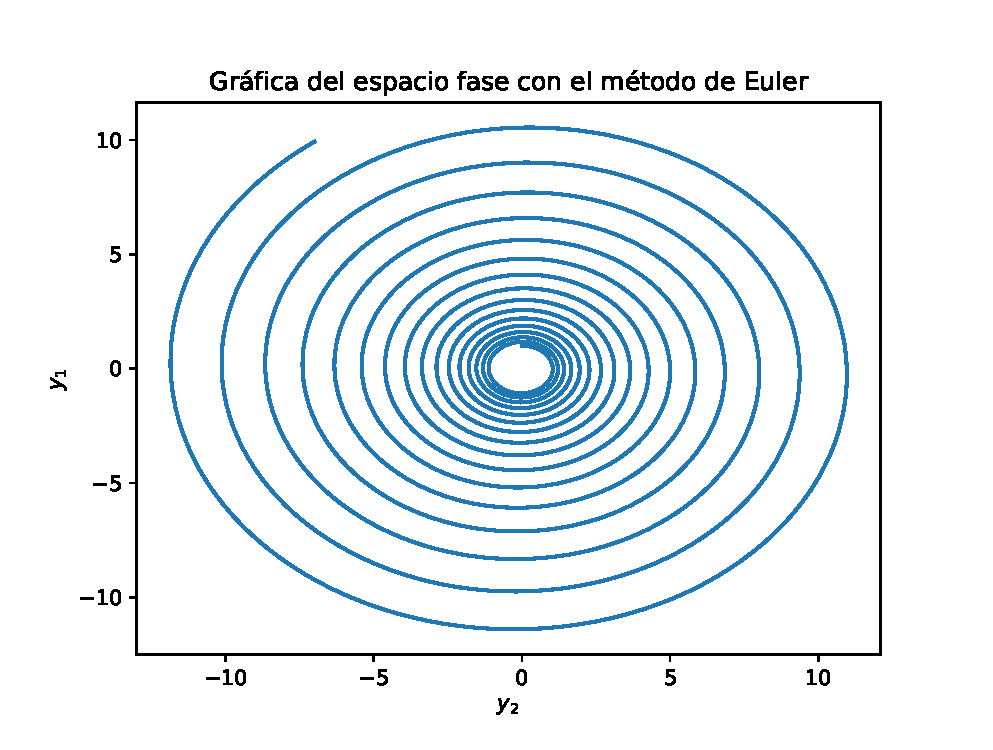
\includegraphics[scale=0.5]{Imagenes/solucion_edo2_Euler_01.eps}
    \caption{Solución numérica obtenida con el método de Euler.}
    \label{fig:figura_12_02}
\end{figure}
\end{frame}
\begin{frame}
\frametitle{Resolviendo con \funcionazul{EulerPC}}
Ahora se modifica dento del ciclo \funcionazul{while} la llamada a la función, ocupando el método predictor-corrector \funcionazul{EulerPC}; se cambia el nombre del archivo de datos, así como en la respectiva instrucción de la rutina de graficación.
\end{frame}
\begin{frame}
\frametitle{Resultado obtenido con el método \funcionazul{EulerPC}}
\begin{figure}[h!]
    \centering
    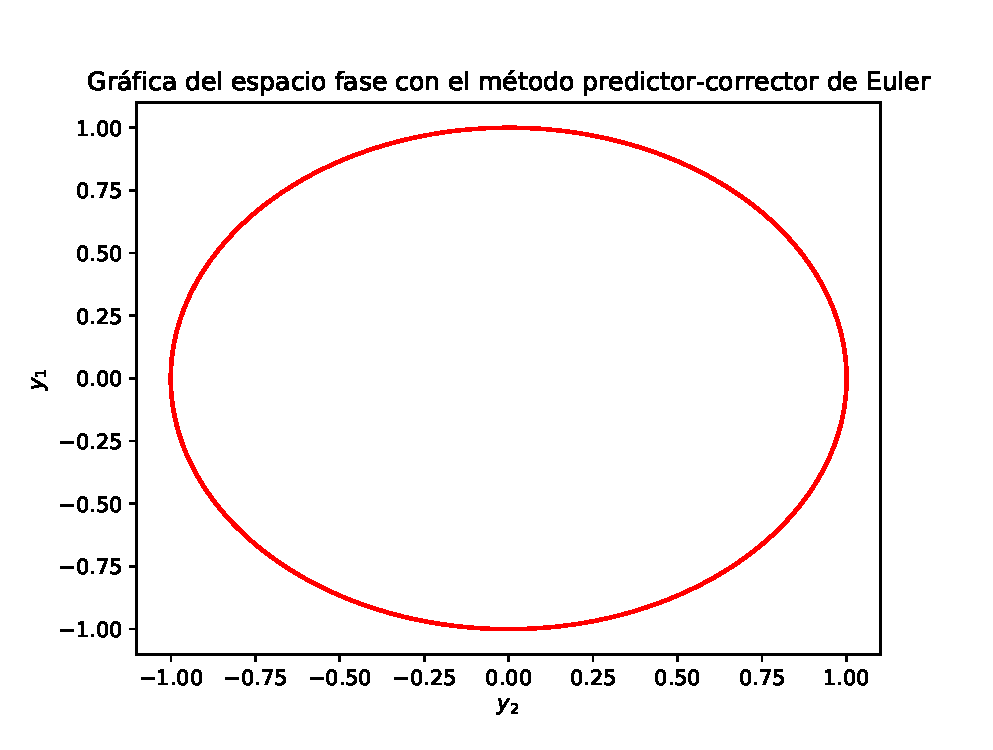
\includegraphics[scale=0.5]{Imagenes/solucion_edo2_Euler_02.eps}
    \caption{Solución numérica obtenida con el método predictor-corrector de Euler.}
    \label{fig:figura_12_03}
\end{figure}
\end{frame}
\begin{frame}
\frametitle{Interpretación y discusión de resultados}
La solución exacta al problema anterior en el caso particular de los valores iniciales 
\begin{align}
y_{1}(0) = 0,  \hspace{1cm} y_{2} (0) = 1
\label{eq:ecuacion_12_22}
\end{align}
es 
\begin{align*}
y_{1}(t) = \sin t \hspace{1cm} y_{2}(t) = \cos t
\end{align*}
y puede se puede comparar fácilmente con la salida numérica producida por el programa.
\end{frame}
\begin{frame}
\frametitle{Interpretación y discusión de resultados}
Una indicación aún más elocuente sobre la estabilidad numérica de la solución es proporcionada por la dependencia de un componente de la solución del otro, concretamente, por la gráfica de $y_{2}$ vs $y_{1}$.
\\
\bigskip
En un caso de propagación estable, se espera que la curva $y_{1} = y_{1} (y_{2})$ sea un círculo cerrado de radio unitario.
\end{frame}
\begin{frame}
\frametitle{Interpretación y discusión de resultados}
Como se puede observar en la figura (\ref{fig:figura_12_02}), el espacio fase que representa la evolución de los perfiles en un lapso de tiempo \funcionazul{tmax = $100$}, obtenido con un tamaño de paso de propagación \funcionazul{h = $0.05$}.
\end{frame}
\begin{frame}
\frametitle{Interpretación y discusión de resultados}
La solución obtenida por el método básico de Euler se aleja progresivamente del esperado comportamiento circular, mientras que, a juzgar por la curva cerrada de radio cercano a $1$, el método de Euler predictor-corrector exhibe una buena estabilidad y precisión.
\end{frame}
\begin{frame}
\frametitle{Interpretación y discusión de resultados}
El método básico de Euler logra un grado de estabilidad comparable al del algoritmo predictor-corrector solo para un tamaño de paso $50$ veces menor, es decir, para \funcionazul{h = $0.001$}.
\\
\bigskip
\textbf{Como ejercicio a cuenta 1}: realiza los ajustes necesarios y envía la gráfica obtenida.
\end{frame}
\subsection{Métodos Runge-Kutta}
\begin{frame}
\frametitle{Métodos Runge-Kutta}
Los métodos Runge-Kutta representan una familia completa de algoritmos para la solución numérica de problemas de valores iniciales para las EDO1 (de primer orden) o sistemas de los mismos.
\\
\bigskip
Debido a su fiabilidad y robustez, los métodos Runge-Kutta han adquirido el estado de \emph{métodos estándar de propósito general} para la integración numérica de una EDO.
\end{frame}
\begin{frame}
\frametitle{Métodos Runge-Kutta}
Los algoritmos de Runge-Kutta son métodos de un solo paso que se inician por sí mismos y requieren solo la evaluación de los lados derechos de las EDO, pero no de sus derivadas.
\end{frame}
\begin{frame}
\frametitle{Métodos Runge-Kutta}
Según la convención general, el método de orden $p$ proporciona soluciones que coinciden con las aproximaciones de orden $\order{h^{p}}$ de la serie de Taylor correspondiente. El aumento del orden se acompaña naturalmente de una precisión superior, pero también de una mayor complejidad de implementación.
\end{frame}
\begin{frame}
\frametitle{Métodos Runge-Kutta}
Consideremos el problema genérico de Cauchy para una EDO1 de primer orden o un sistema de EDO1:
\begin{align}
\ptilde{y} = f(t, y), \hspace{1cm} y(t_{0}) = y_{0}
\label{eq:ecuacion_12_23}
\end{align}
\end{frame}
\begin{frame}
\frametitle{Métodos Runge-Kutta}
La propagación de la solución $y(t)$ de $t_{m}$ a $t_{m+1}$ se logra mediante una expansión en serie de Taylor:
\begin{align}
\begin{aligned}
y_{m+1} &= y_{m} + h \, f(t_{m}, y_{m}) + \\[0.5em]
&+ \dfrac{h^{2}}{2} \left[ \pdv{f}{t} + f \, \pdv{f}{y} \right]_{t_{m}, y_{m}} + \ldots
\end{aligned}
\label{eq:ecuacion_12_24}
\end{align}
\end{frame}
\begin{frame}
\frametitle{Inconveniente del método}
Mantener una gran cantidad de términos en esta serie, con el fin de aumentar la precisión, no es práctico, debido al rápido aumento de la complejidad de las derivadas involucradas de la función del lado derecho $f(t, y)$.
\end{frame}
\begin{frame}
\frametitle{Mejora del método}
Los métodos de Runge-Kutta siguen en cambio otra idea principal: construir soluciones dependiendo de los valores de $f (t, y)$, pero no de sus derivadas, y cuyas representaciones de series de potencia en $h$ deberían ser equivalentes a la expansión exacta (ec. \ref{eq:ecuacion_12_24}) hasta los términos más altos posibles, independientemente de la función particular $f (t, y)$.
\end{frame}
\begin{frame}
\frametitle{Construcción del método}
Representamos $y_{m+1}$ como una combinación lineal
\begin{align}
y_{m+1} = y_{m} + \sum_{i=1}^{p} w_{i} \, k_{i}
\label{eq:ecuacion_12_25}
\end{align}
donde los $w_{i}$ son los pesos y las $k_{i}$ son los valores proporcionales a $f(t, y)$.
\begin{align*}
k_{i} = h \, f(\xi_{i}, \eta_{i})
\end{align*}
\end{frame}
\begin{frame}
\frametitle{Construcción del método}
Para $p$ pares de argumentos particulares de la vecindad de $t_{m}$ y $y_{m}$:
\begin{align}
\begin{cases}
\xi_{i} = t_{m} + \alpha_{i} \, h \\[0.5em]
\eta_{i} = y_{m} + \displaystyle \sum_{j=1}^{i-1} \beta_{ij} \, k_{j}
\end{cases}
\label{eq:ecuacion_12_26}
\end{align}
las $\alpha_{i}, \beta_{i}$ y $w_{i}$ son parámetros ajustables, que deben determinarse para maximizar la relación entre la combinación lineal (ec. \ref{eq:ecuacion_12_25}) y la serie Taylor (ec. \ref{eq:ecuacion_12_24}).
\end{frame}
\begin{frame}
\frametitle{Construcción del método}
Sin pérdida de generalidad, podemos considerar en todos los casos:
\begin{align}
\alpha_{1} = 0 \hspace{0.5cm} \beta_{11} = 0, \hspace{0.5cm} \xi_{1} = t_{m} \hspace{0.5cm} \eta_{1} = y_{m}
\label{eq:ecuacion_12_27}
\end{align}
lo cual garantiza que $h \, f(t_{m}, y_{m})$ es siempre el primer término en cualquier propagador Runge-Kutta (ec. \ref{eq:ecuacion_12_25}).
\end{frame}
\begin{frame}
\frametitle{Construcción del método}
Entonces tenemos:
\begin{align}
\begin{cases}
k_{1} = h \, f(t_{m}, y_{m}), \\[0.5em]
k_{2} = h \, f(t_{m} + \alpha_{2} \, h, y_{m} + \beta_{21} \, k_{1}), \\[0.5em]
k_{2} = h \, f(t_{m} + \alpha_{3} \, h, y_{m} + \beta_{31} \, k_{1} + \beta_{32} \, k_{2}), \\[0.5em]
\ldots \ldots
\end{cases}
\label{eq:ecuacion_12_28}
\end{align}
\end{frame}
\begin{frame}
\frametitle{Construcción del método}
Las relaciones anteriores revelan el carácter algorítmico explícito de los métodos Runge-Kutta, lo que significa que las diversas cantidades se calculan de manera directa basándose solo en cantidades ya disponibles.
\end{frame}
\begin{frame}
\frametitle{Construcción del método}
Determinemos a continuación los parámetros $\alpha_{i}, \beta_{i}$ y $w_{i}$ para métodos de varios órdenes $p$, de tal manera que la expansión de la fórmula de propagación (ec. \ref{eq:ecuacion_12_25}) en potencias de $h$ sea equivalente a la aproximación de orden $\order{h^{p}}$ de la solución en series de Taylor (ec. \ref{eq:ecuacion_12_24}).
\end{frame}
\begin{frame}
\frametitle{Método Runge-Kutta de primer orden}
Para $p = 1$, tenemos que
\begin{align}
y_{m+1} = y_{m} + h \, f(t_{m}, y_{m})
\label{eq:ecuacion_12_29}
\end{align}
y se recupera la fórmula de Euler, que resulta ser idéntica al \textoazul{método Runge-Kutta de primer orden (RK1)}.
\end{frame}
\begin{frame}
\frametitle{Método Runge-Kutta de segundo orden}
Para $p = 2$, la fórmula del propagador (\ref{eq:ecuacion_12_25}) y los coeficientes (\ref{eq:ecuacion_12_28}) toman la forma particular
\begin{align*}
y_{m+1} = y_{m} +  w_{1} \, k_{1} + w_{2} \, k_{2}
\end{align*}
y respectivamente
\begin{align*}
\begin{cases}
k_{1} = h \, f(t_{m}, y_{m}) \\[0.5em]
k_{2} = h \, f(t_{m} + \alpha_{2} \, h, y_{m} + \beta_{21} \, k_{1})
\end{cases}
\end{align*}
\end{frame}
\begin{frame}
\frametitle{Método Runge-Kutta de segundo orden}
Combinando esas relaciones se obtiene
\begin{align*}
y_{m+1} &= y_{m} +  w_{1} \, h \, f(t_{m}, y_{m}) + \\
&+ w_{2} \, h \, f(t_{m} + \alpha_{2} \, h, y_{m} + \beta_{21} \, h \, f(t_{m}, y_{m}))
\end{align*}
\end{frame}
\begin{frame}
\frametitle{Método Runge-Kutta de segundo orden}
Expandiendo el último término en una serie de potencias en $h$, se obtiene:
\begin{align}
\begin{aligned}
y_{m+1} &= y_{m} +  w_{1} \, h \, f(t_{m}, y_{m}) + \\
&+ h^{2} \left[ w_{2} \, \alpha_{2} \, \pdv{f}{t} + w_{2} \, \beta_{21} \, \pdv{f}{y} \right]_{t_{m}, y_{m}}
\end{aligned}
\label{eq:ecuacion_12_30}
\end{align}
\end{frame}
\begin{frame}
\frametitle{Método Runge-Kutta de segundo orden}
Comparando ésta fórmula con la serie de Taylor (ec. \ref{eq:ecuacion_12_24}), e igualando los coeficientes con la misma potencia de $h$, nos lleva a
\begin{align*}
\begin{cases}
w_{1} + w_{2} = 1 \\[0.5em]
w_{2} \, \alpha_{2} = 1/2 \\[0.5em]
w_{2} \, \beta_{21} = 1/2
\end{cases}
\end{align*}
\pause
Este sistema no lineal indeterminado con cuatro incógnitas que no tiene una solución única.
\end{frame}
\begin{frame}
\frametitle{Método Runge-Kutta de segundo orden}
Observando que es necesario tener $w_{2} \neq 0$, una opción simple a la mano, que también favorece la simetría, es $w_{2} = 1/2$ y por lo tanto resulta:
\begin{align*}
\alpha_{2} &= \beta_{21} =  1 \\[0.5em]
w_{1} &= w_{2} = 1/2
\end{align*}
\end{frame}
\begin{frame}
\frametitle{Método Runge-Kutta de segundo orden}
Con esos coeficientes, la fórmula para el \textoazul{método de Runge-Kutta de segundo orden (RK2)} es:
\begin{align}
y_{m+1} = y_{m} + \dfrac{1}{2} (k_{1} + k_{2}) + \order{h^{3}}
\label{eq:ecuacion_12_31}
\end{align}
con
\begin{align}
\begin{cases}
k_{1} = h \, f(t_{m}, y_{m}) \\[0.5em]
k_{2} = h \, f(t_{m} + h, y_{m} + k_{1})
\end{cases}
\label{eq:ecuacion_12_32}
\end{align}
\end{frame}
\begin{frame}
\frametitle{Método Runge-Kutta de segundo orden}
Combinando las relaciones anteriores, tenemos el resultado:
\begin{align}
\begin{aligned}
y_{m+1} = y_{m} &+ \dfrac{h}{2} \left[ f(t_{m}, y_{m}) + \right. \\ 
&\left. + f(t_{m} + h, y_{m} + h \, f(t_{m}, y_{m})) \right] 
\end{aligned}
\label{eq:ecuacion_12_33}
\end{align}
se recupera el método predictor-corrector de Euler, con el predictor dentro de la fórmula del corrector.
\end{frame}
\subsection{Método Runge-Kutta de 4o. orden}
\begin{frame}
\frametitle{Método Runge-Kutta de 4o. orden}
La variante más importante y ampliamente utilizada es el \textoazul{método Runge-Kutta de cuarto orden (RK4)} $(p = 4)$, ya que ofrece un buen control de error de truncamiento local y una forma funcional fácilmente implementable.
\end{frame}
\begin{frame}
\frametitle{Método Runge-Kutta de 4o. orden}
Siguiendo el mismo razonamiento para determinar los coeficientes $\alpha_{i}, \beta_{i}$ y $w_{i}$ como en el caso $p = 2$, resulta un sistema no lineal de $10$ ecuaciones con $13$ incógnitas, que, al estar indeterminado, no tiene una solución única.
\\
\bigskip
Se utilizan varios conjuntos de coeficientes, aunque se prefieren aquellos que presentan simplicidad o favorecen el uso eficiente del almacenamiento.
\end{frame}
\begin{frame}
\frametitle{Método Runge-Kutta de 4o. orden}
La variante comúnmente empleada del método Runge-Kutta de cuarto orden se define por las relaciones:
\fontsize{12}{12}\selectfont
\begin{align}
y_{m+1} &= y_{m} + \dfrac{1}{6} \big( k_{1} + 2 \, k_{2} + 2 \, k_{3} + k_{4} \big) + \order{h^{5}} \label{eq:ecuacion_12_34} \\[1em]
&\begin{cases}
k_{1} = h \, f(t_{m}, y_{m}) \\[0.5em]
k_{2} = h \, f(t_{m} + h/2, y_{m} + k_{1}/2) \\[0.5em]
k_{3} = h \, f(t_{m} + h/2, y_{m} + k_{2}/2) \\[0.5em]
k_{4} = h \, f(t_{m} + h, y_{m} + k_{3})
\end{cases} \label{eq:ecuacion_12_35}
\end{align}
\end{frame}
\begin{frame}
\frametitle{Método RK4}
El método implica en cada paso de propagación cuatro evaluaciones de la función del lado derecho $f(t, y)$ de la EDO.
\\
\bigskip
El error de truncamiento correspondiente refleja la omisión de los términos del orden $\order{(h^{5}}$:
\begin{align}
\Delta_{m+1} \sim K \, h^{5}
\end{align}
\end{frame}
\begin{frame}
\frametitle{Método RK4}
Cabe destacar que, para una función del lado derecho $f$ independiente de $y$, la ecuación diferencial se convierte en la integral simple de $f$ en el intervalo $[t_{m}, t_{m} + h]$, y el método RK4 se vuelve equivalente con la regla de Simpson:
\end{frame}
\begin{frame}
\frametitle{Método RK4}
\begin{align*}
y_{m+1} = y_{m} + \dfrac{h}{6} \big[ f(t_{m}) + 4 \, f(t_{m} + h/2) + f(t_{m} + h) \big]
\end{align*}
Los valores dobles de los coeficientes estándar de la regla de Simpson $(1/3, 4/3, 1/3)$ vienen de la definición de la longitud del intervalo de integración como $2 \, h$ en lugar de $h$.
\end{frame}
\begin{frame}
\frametitle{Método RK4}
Además de la precisión satisfactoria y la implementación simple, al ser un algoritmo explícito de un solo paso, el método RK4 se destaca también por su capacidad de inicio automático.
\\
\bigskip
El sistema de solución RK4 también es útil para proporcionar valores iniciales para métodos de varios pasos más precisos, pero no de inicio automático.
\end{frame}
\begin{frame}
\frametitle{Método RK4}
Aprovechando la estructura simple de los coeficientes $k_{1}, k_{2}, k_{3}, k_{4}$ del método RK4 (ecs. \ref{eq:ecuacion_12_34}, \ref{eq:ecuacion_12_35}), para un sistema de $n$ EDO1, es conveniente referirse explícitamente a los valores de las funciones del lado derecho $f_{i}$:
\end{frame}
\begin{frame}
\frametitle{Método RK4}
Referencia explícita a los valores:
\fontsize{12}{12}\selectfont
\begin{align}
y_{m+1} &= y_{m,i} + \dfrac{h}{6} \big( f_{1,i} + 2 \, f_{2,i} + 2 \, f_{3, i} + f_{4, i} \big), \hspace{0.5cm} i = 1, 2, \ldots, n \label{eq:ecuacion_12_37} \\[0.5em]
&\begin{cases}
f_{1, i} = f_{i}(t_{m}, \left\{ y_{m, i} \right\}), \\[0.5em]
f_{2, i} = f_{i}(t_{m} + h/2, \left\{ y_{m, i} + (h/2) \, f_{1,i} \right\}), \\[0.5em]
f_{3, i} = f_{i}(t_{m} + h/2, \left\{ y_{m, i} + (h/2) \, f_{2,i} \right\}), \\[0.5em]
f_{4, i} = f_{i}(t_{m} + h, \left\{ y_{m, i} + h \, f_{3,i} \right\})
\end{cases} \label{eq:ecuacion_12_38}
\end{align}
\end{frame}
\begin{frame}
\frametitle{Método RK4}
Las llaves indican el conjunto completo de argumentos para todos los componentes de la solución (ejecutando todos los valores de $i$).
\\
\bigskip
Obviamente, el formalismo también se puede aplicar para resolver problemas de Cauchy para EDO de orden superior, transformando primero la ecuación en un sistema de EDO de primer orden.
\end{frame}
\begin{frame}
\frametitle{Propuesta de código para RK4}
La rutina \funcionazul{RungeKutta} representa el código para el algoritmo descrito para resolver un problema Cauchy \enquote{elemental} para un sistema de EDO1.
\\
\bigskip
Concretamente, la rutina realiza en cada llamada una propagación en un solo paso de la solución conocida $(y_{m, i}, \hspace{0.1cm} i = 1, 2, \ldots, n)$ de $t_{m}$ a $t_{m + 1} = t_{m} + h$, generando componentes actualizados $y_{m + 1}$, de acuerdo con las ecs. \ref{eq:ecuacion_12_37}-\ref{eq:ecuacion_12_38}.
\end{frame}
\begin{frame}
\frametitle{Propuesta de código para RK4}
Se supone que el arreglo $y$ contiene en la entrada los $n$ componentes de la solución inicial, que se reemplazan al salir por sus valores propagados con un tamaño de paso $h \, t$.
\end{frame}
\begin{frame}
\frametitle{Propuesta de código para RK4}
La rutina llama a la función proporcionada por el usuario \funcionazul{Func} que devuelve los valores $f_{1,i}, f_{2,i}, f_{3,i},$ y $f_{4,i}$ de las funciones del lado derecho $f_{i} (t,  y_{1}, \ldots, y_{n}), i = 1, 2, \ldots$. Los arreglos correspondientes $f_{1}, f_{2}, f_{3}, f_{4}$ se asignan en la primera entrada en la rutina.
\end{frame}
\begin{frame}[allowframebreaks, fragile]
\frametitle{Código para el método RK4}
\begin{lstlisting}[caption=Código para el método RK4, style=codigopython]
def RungeKutta(t, ht, y, n, Func):
    fA_1_B = [0]*(n+1); fA_2_B = [0]*(n+1)
    fA_3_B = [0]*(n+1); fA_4_B = [0]*(n+1)
    yt = [0]*(n+1)
 
    htA_2_B = ht/2e0
    Func(t, y, fA_1_B)
    for i in range(1,n+1): yt[i] = y[i] + htA_2_B*fA_1_B[i]
    Func(t+htA_2_B, yt, fA_2_B)
    for i in range(1,n+1): yt[i] = y[i] + htA_2_B*fA_2_B[i]
    Func(t+htA_2_B, yt, fA_3_B)
    for i in range(1, n+1): yt[i] = y[i] + ht *fA_3_B[i]
    Func(t+ht, yt, fA_4_B)
 
    hA_6_B = ht/6e0
    for i in range(1, n+1): y[i] += hA_6_B*(fA_1_B[i] + 2*(fA_2_B[i] + fA_3_B[i]) + fA_4_B[i]) 
\end{lstlisting}
\end{frame}
\begin{frame}
\frametitle{Ejemplo para el método RK4}
Con el siguiente ejemplo veremos la funcionalidad del \textoazul{método RK4}, consideremos el problema no lineal del péndulo.
\\
\bigskip
\pause
Para un péndulo de longitud constante $\ell$, la ecuación de movimiento para el desplazamiento angular $u$ con respecto a la vertical pasando por un punto de suspensión, es una EDO2 no lineal:
\begin{align}
\stilde{u} = - \dfrac{g}{\ell} \, \sin u
\label{eq:ecuacion_12_39}
\end{align}
\end{frame}
\begin{frame}
\frametitle{Condiciones para la EDO2 no lineal}
Este problema normalmente se resuelve con las condiciones iniciales para el desplazamiento inicial y la derivada en $t = 0$:
\begin{align}
u(0) = u_{0} \hspace{0.5cm} \ptilde{u}(0) = 0
\label{eq:ecuacion_12_40}
\end{align}
\end{frame}
\begin{frame}
\frametitle{Aproximación con pequeñas amplitudes}
Para oscilaciones de \emph{pequeñas amplitudes} $u_{0}$, el lado derecho de la ec (\ref{eq:ecuacion_12_39}) se puede \enquote{linealizar} usando la aproximación $\sin u \equiv u$ y la correspondiente \emph{solución armónica}
\begin{align*}
u(t) = u_{0} \, \cos \left( \dfrac{2 \, \pi}{T_{0}} \, t \right), \hspace{0.5cm} T_{0} = 2 \, \pi \sqrt{\dfrac{\ell}{g}}
\end{align*}
que se caracteriza por un período independiente de la amplitud $T_{0}$.
\end{frame}
\begin{frame}
\frametitle{Período para oscilaciones arbitrarias}
Para oscilaciones de amplitud arbitraria, se puede demostrar que el período depende en gran medida del desplazamiento angular inicial $u_{0} \in [-\pi, \pi]$:
\begin{align}
T = T_{0} \, \dfrac{2}{\pi} \, K \, \left( \sin^{2} \dfrac{u_{0}}{2} \right)
\label{eq:ecuacoin_12_41}
\end{align}
\end{frame}
\begin{frame}
\frametitle{Integral elíptica de primera clase}
Donde $K(m)$ es la integral elíptica de primera clase, definida por
\begin{align}
K(m) = \int_{0}^{1} \dfrac{\dd{z}}{\sqrt{(1 - z^{2})(1 - m \, z^{2})}}
\label{eq:ecuacion_12_42}
\end{align}
\end{frame}
\begin{frame}
\frametitle{Ajuste de la EDO a la notación}
Para resolver numéricamente el problema del péndulo no lineal con alguno de los métodos RK, debemos primero de ajustar la EDO2 a un sistema de EDO1:
\begin{align*}
\begin{cases}
\ptilde{u}_{1} = u_{2} \\[0.5em]
\ptilde{u}_{2} = -\left( \dfrac{g}{\ell} \right) \, \sin (u_{1}) - k \, u_{2}
\end{cases}
\hspace{0.5cm}
\begin{cases}
u_{1}(0) = u_{0} \\[0.5em]
u_{2}(0) = 0
\end{cases}
\end{align*}
\end{frame}
\begin{frame}
\frametitle{Ajuste de la EDO a la notación}
Además del modelo inicial, aquí, también se prevé un término de amortiguamiento dependiente de la velocidad $(u_{2} = \ptilde{u})$ con un coeficiente de velocidad $k$.
\end{frame}
\begin{frame}
\frametitle{Sobre el código para la solución}
En el siguiente código, los términos del lado derecho de las EDO1 anteriores se codifican dentro de la función de usuario \funcionazul{Func}.
\\
\bigskip
Dado que \funcionazul{Func} tiene que cumplir con la lista de parámetros esperada por la rutina \funcionazul{RungeKutta}, recibe las cantidades específicas del problema $\ell$ y $k$ a través de los parámetros globales \funcionazul{l} y \funcionazul{k}, que son valores asignados en el programa principal.
\end{frame}
\begin{frame}
\frametitle{Sobre el código para la solución}
El programa principal calcula el período de oscilación mediante un enfoque elemental pero seguro. Específicamente, el ciclo de propagación identifica los ceros primero y último de la solución $u_{1} (t)$ por los cambios de signo, y cuenta los medios períodos abarcados.
\\
\bigskip
El período entonces resulta dividiendo el lapso de tiempo entre los ceros extremos por el número de medios períodos.
\end{frame}
\begin{frame}[allowframebreaks, fragile]
\frametitle{Código con \python}
\begin{lstlisting}[caption=Código para el problema del péndulo no lineal, style=codigopython]
import numpy as np
from Metodos_Directos import RungeKutta

g = 9.81e0

def Func(t, u, f):
    f[1] =  u[2]
    f[2] = -g/l * np.sin(u[1]) - k * u[2]

l = 1e0
k = 0e0
uA_0_B = 0.5e0*np.pi
duA_0_B = 0e0
tmax = 20e0
ht = 0.001e0

n = 2
u = [0]*(n+1)

salida = open("pendulo.txt","w")
salida.write("t \t u \t du\n")

t = 0e0
u[1] = uA_0_B; u[2] = duA_0_B
salida.write(("{0:10.5f} \t {1:10.5f} \t {2:10.5f}\n").format(t, u[1], u[2]))

nT = 0
tA_1_B = tA_2_B = 0e0
us = u[1]
while (t+ht <= tmax):
    RungeKutta(t, ht, u, n, Func)
    t += ht

    if (u[1]*us < 0e0):
        if (tA_1_B == 0): tA_1_B = t
        else: tA_2_B = t; nT += 1
    us = u[1]

    salida.write(("{0:10.5f} \t {1:10.5f} \t {2:10.5f}\n").format(t, u[1], u[2]))

T = 2e0*(tA_2_B-tA_1_B) / nT
TA_0_B = 2e0*np.pi*np.sqrt(l/g)
print("uA_0_B = {0:7.5f} \t T/TA_0_B = {1:7.5f}".format(uA_0_B, T/TA_0_B))

salida.close()
\end{lstlisting}
\end{frame}
\begin{frame}
\frametitle{Resultado gráfico de la solución}
Implementamos una rutina para recuperar los datos del archivo \emph{pendulo.txt}, (siguiendo el mismo procedimiento que usamos anteriormente con \funcionazul{numpy.loadtxt}) para graficar $u$ vs $t$:
\end{frame}
\begin{frame}
\frametitle{Resultado gráfico de la solución}
\begin{figure}[h!]
    \centering
    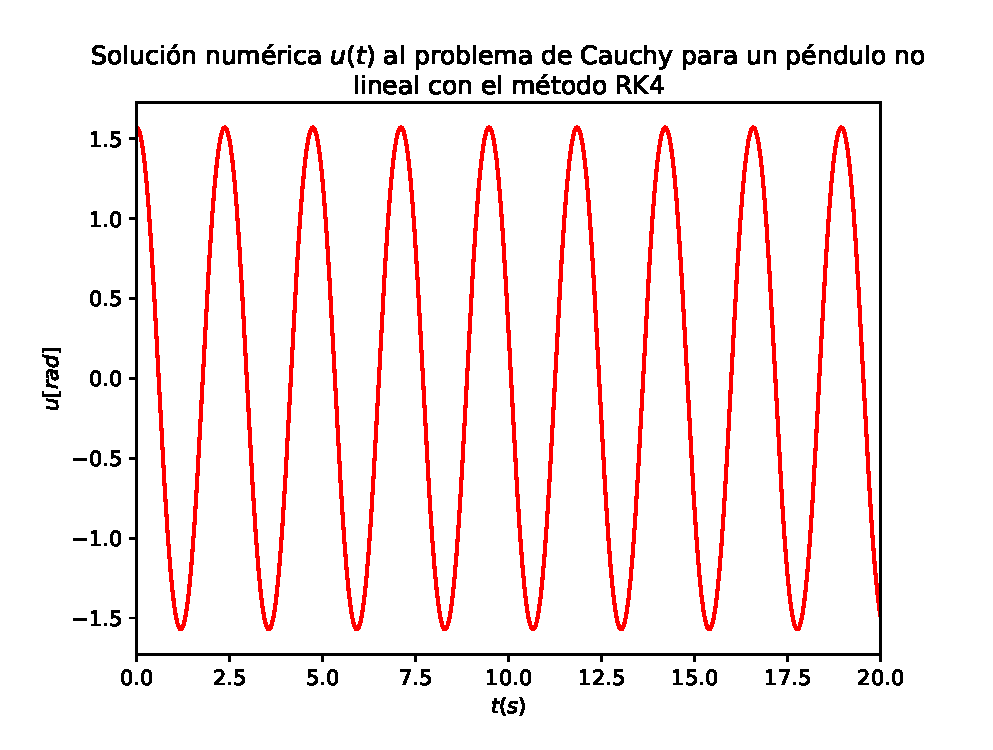
\includegraphics[scale=0.5]{Imagenes/metodo_RK4_pendulo_01.eps}
    \caption{Solución numérica $u(t)$ para el problema de Cauchy con el método RK4.}
    \label{fig_figura_12_pendulo01}
\end{figure}
\end{frame}
\begin{frame}
\frametitle{Gráfica del espacio fase del péndulo}
Con el fin de extender el análisis del resultado del método RK4, graficamos el espacio fase de la trayectoria del péndulo, $\ptilde{u}$ vs $u$:
\end{frame}
\begin{frame}
\frametitle{Gráfica del espacio fase del péndulo}
\begin{figure}[h!]
    \centering
    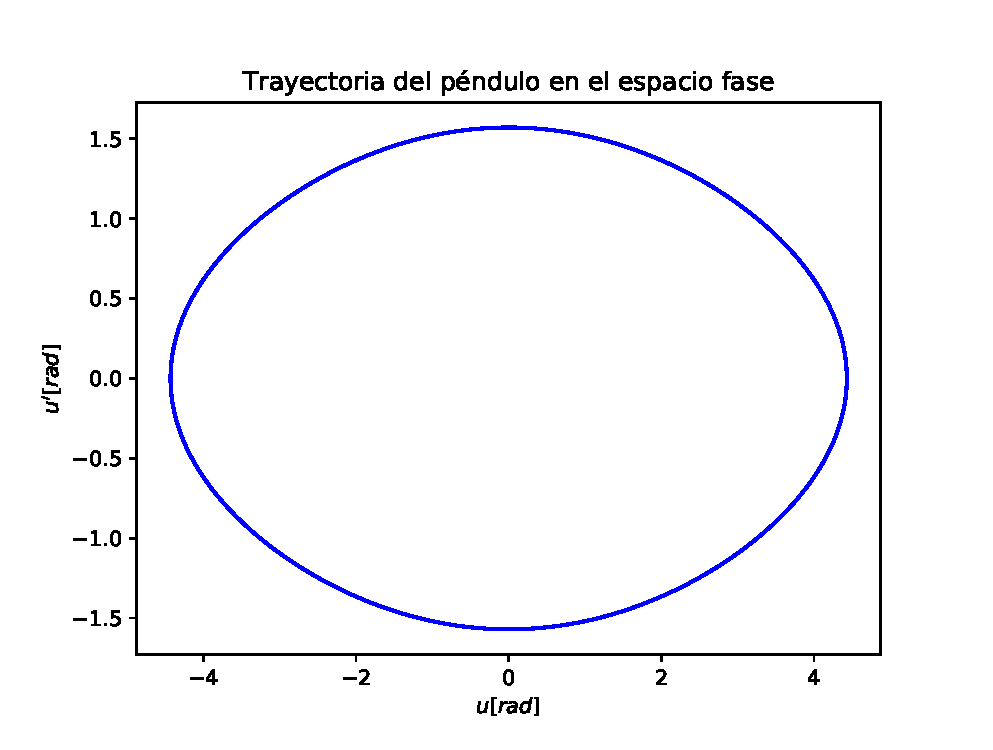
\includegraphics[scale=0.5]{Imagenes/metodo_RK4_pendulo_02.eps}
    \caption{Espacio fase del péndulo no lineal.}
    \label{fig_figura_12_pendulo02}
\end{figure}
\end{frame}
\begin{frame}
\frametitle{Una discusión mayor sobre los resultados}
Con la solución obtenida contamos con una referencia básica, pero es necesario extender la discusión sobre el problema del péndulo no lineal.
\\
\bigskip
Si hacemos un cambio en el valor del desplazamiento angular inicial $u_{0}$ y comparamos las gráficas veremos un resultado interesante:
\end{frame}
\begin{frame}
\frametitle{Compración de resultados}
\begin{figure}[h!]
    \centering
    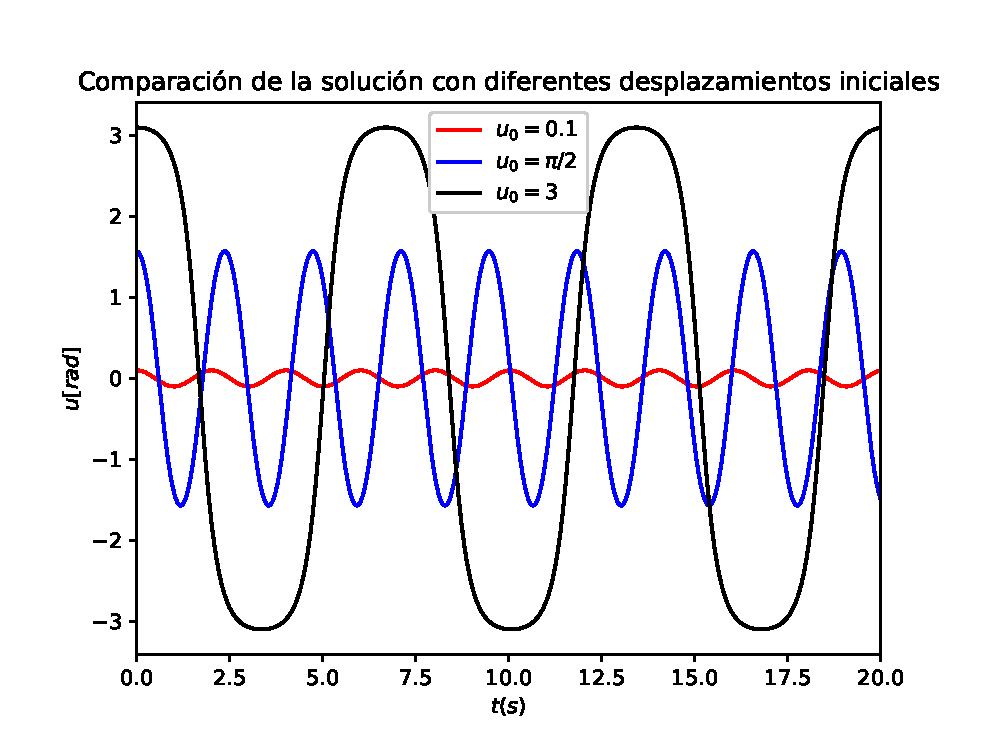
\includegraphics[scale=0.5]{Imagenes/metodo_RK4_pendulo_03.eps}
    \caption{Soluciones con varios desplazamientos angulares $u_{0}$.}
    \label{fig_figura_12_pendulo03}
\end{figure}
\end{frame}
\begin{frame}
\frametitle{Comparación de resultados}
La figura \ref{fig_figura_12_pendulo03} muestra las \emph{tremendas} diferencias entre las soluciones dependientes del tiempo obtenidas al ejecutar el código para los desplazamientos angulares iniciales $u_{0} = 0.01, \pi / 2, 3.1$, en ausencia de fuerzas de fricción $(k = 0)$.
\end{frame}
\begin{frame}
\frametitle{Ejercicio a cuenta 2}
Como ejercicio a cuenta debes de reproducir la gráfica anterior utilizando el código RK4 que se presentó para $u_{0} = \pi/2$, incorporando los otros valores $u_{0} = 0.1, 3.1$.
\\
\bigskip
La gráfica se debe de obtener en una sola ejecución, por lo que debes de ajustar el código, para generar los archivos de datos y posteriormente, ajustar la rutina de graficación.
\end{frame}
\begin{frame}
\frametitle{Ejercicio a cuenta 3}
Resuelve los siguientes problemas en $0 \leq t \leq 5$ mediante el método de Euler con $h = 0.01$.
\setbeamercolor{item projected}{bg=blue!70!black,fg=yellow}
\setbeamertemplate{enumerate items}[circle]
\begin{enumerate}
\item $\ptilde{y} + t \, y = 1 \hspace{1.5cm} y(0)=1$
\item $\ptilde{y} + 3 \, y = e^{-t} \hspace{1.5cm} y(0)=1$
\item $\ptilde{y}= (t^{2} - y) \hspace{1.5cm} y(0)=0.5$
\item $\ptilde{y} + y \abs{y} = 0 \hspace{1.5cm} y(0)=1$
\item $\ptilde{y} + \abs{y}^{1/2} = \sin(t) \hspace{1.5cm} y(0)=1$
\end{enumerate}
Evalúa los errores comparando el resultado con los valores exactos.
\end{frame}
\begin{frame}
\frametitle{Ejercicio a cuenta 4}
Se dispara un proyectil al aire con un ángulo de $\ang{45}$ con respecto al suelo, con $u = v = \SI{150}{\meter\per\second}$, donde $u$ y $v$ son las velocidades horizontal y vertical, respectivamente. Las ecuaciones de movimiento están dadas por
\begin{align*}
\ptilde{u} & = -c \, V \, u, \hspace{1.5cm} u(0) = \SI{150}{\meter\per\second} \\[0.5em]
\ptilde{v} & = -g - c \, V \, v, \hspace{1.5cm} v(0) = \SI{150}{\meter\per\second}
\end{align*}
donde $u$ y $v$ son funciones del tiempo, $u = u(t)$ y $v = v(t)$, además
\end{frame}
\begin{frame}
\frametitle{Ejercicio a cuenta 4}
Además:
\begin{align*}
V & = \sqrt{u^{2} + v^{2}} \\[0.5em]
c & = 0.005  \hspace{1cm} \text{(coeficiente de arrastre)} \\[0.5em]
g & = \SI{9.9}{\meter\per\square\second}
\end{align*}
\end{frame}
\begin{frame}
\frametitle{Ejercicio a cuenta 4}
Las ecuaciones de movimiento se pueden resolver mediante alguno de los métodos de Runge-Kutta. La trayectoria del proyectil se puede determinar al integrar
\begin{align*}
\ptilde{x} = u \hspace{1cm} \mbox{y} \hspace{1cm} \ptilde{y} = v
\end{align*}
o bien
\begin{align*}
x & = \int^{t}_{0} u(t^{\prime}) \dd{t^{\prime}} \\[0.5em]
y & = \int^{t}_{0} v(t^{\prime}) \dd{t^{\prime}}
\end{align*}
\end{frame}
\begin{frame}
\frametitle{Ejercicio a cuenta 4}
\setbeamercolor{item projected}{bg=blue!70!black,fg=yellow}
\setbeamertemplate{enumerate items}[circle]
\begin{enumerate}[<+->]
\item Resuelve el ejercicio usando el método RK2 y grafica la trayectoria del proyectil.
\item Implementa la solución ahora con el método RK4, grafica la trayectoria del proyectil.
\item Discute tus resultados.
\end{enumerate}
\end{frame}
\begin{frame}
\frametitle{Ejercicio a cuenta 5}
El movimiento del sistema de masas que se muestra en la siguiente figura, está dado por:
\begin{align*}
\stilde{y} + 2 \, \zeta \, \omega \, \ptilde{y} + \omega^{2} \, y = \dfrac{F(t)}{M}
\end{align*}
donde:
\end{frame}
\begin{frame}
\frametitle{Ejercicio a cuenta 5}
Donde \\
$\omega = \left( \dfrac{k}{M} \right)^{2}$ (frecuencia natural sin amortiguamiento, $[s^{-1}]$) \\
$\zeta = \dfrac{c}{2 \, M \, \omega} = 0.5$ (factor de amortiguamiento) \\
$k = 3.2$ (constante del resorte, $\big[ \dfrac{kg}{s^{2}} \big]$) \\
$M = 5$ (masa, [kg]) \\
$F(t) = 0$ (fuerza, [Newtons])
\end{frame}
\begin{frame}
\frametitle{Ejercicio a cuenta 5}
\begin{figure}[h!]
	\centering
	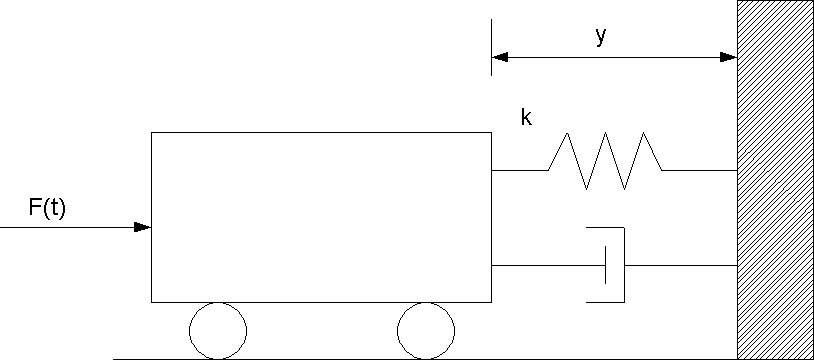
\includegraphics[scale=0.4]{Imagenes/Figura01.png}  
    \caption{Sistema masa-resorte.}
\end{figure}
\end{frame}
\begin{frame}
\frametitle{Ejercicio a cuenta 5}
\setbeamercolor{item projected}{bg=blue!70!black,fg=yellow}
\setbeamertemplate{enumerate items}[circle]
\begin{enumerate}[<+->]
\item Si $F(t)$ es una función escalonada de magnitud $F_{0} = \SI{1}{\newton}$, cuya duración es de $1$ segundo, determina el movimiento de la masa para $0 < t < 10$ segundos usando el método RK4.
\seti
\end{enumerate}
\end{frame}
\begin{frame}
\frametitle{Ejercicio a cuenta 5}
\setbeamercolor{item projected}{bg=blue!70!black,fg=yellow}
\setbeamertemplate{enumerate items}[circle]
\begin{enumerate}[<+->]
\conti
\item Determina la respuesta y carga dinámica del sistema amortiguado sujeto ahora a un pulso de fuerza triangular
\begin{align*}
F(t) =
\begin{cases}
2 \, F_{0} \, t,  & 0 \leq t \leq 1 \, s\\
2 \, F_{0} (1 - t), & 1 \leq t \leq 2 \, s\\
0, & t > 2 \, s
\end{cases}
\end{align*}
Donde $F_{0} = 1$ (fuerza), resuelve con RK4.
\end{enumerate}
\end{frame}
% \\
% \item  Utiliza el m\'{e}todo RK4.
% \end{frame}
% \end{frame}
% \begin{frame}[fragile]
% \frametitle{Ejercicio}
% El circuito que se muestra, tiene una autoinductancia de $L = \SI{50}{\henry}$, una resistencia de $R = \SI{20}{\ohm}$, y una fuente de $V = \SI{10}{\volt}$.
% \begin{center}
% \begin{circuitikz}[scale=0.8]
% \draw
%     (0,0)
%         to[battery1, l=$V$] ++(0,4)
%         to[short] ++(1,0)
%         to[L, l^=$L_{1}$] ++(1.5,0)
%         to[short] ++(1,0) coordinate (A)
%         to[short] ++(1,0)
%         to[R, l^=$R_{2}$] ++(1.5,0)
%         to[short] ++(1,0)
%         to[L, l^=$L_{2}$] ++(0,-4)--(1,0)
%         to[cspst, o-o] ++(0.8,0) -- (0,0)
%         (A)
%         to[short] ++(0,-0.5)
%         to[R, l^=$R_{1}$] ++(0,-1.5)
%         to[C, l^=$C$] ++(0,-2);
% \end{circuitikz}
% \end{center}
% \end{frame}
% \begin{frame}
% En $t = 0$, la corriente $I(t)$ satisface
% \begin{align*}
% L \, \dv{I(t)}{t} \, I(t) + R \, I(t) = V, \hspace{1cm} I(0) = 0
% \end{align*}
% Usando el \funcionazul{método RK2}, calcula la corriente para $0 \leq t \leq 10$ segundos, con $h = 0.1$
% \end{frame}
% \begin{frame}
% Se reescribe la ecuación como
% \[\dfrac{d}{dt} I = -\dfrac{R}{L} I + \dfrac{V}{L} = f(I,t)\]
% Aplicando el método RK2, tenemos
% \begin{eqnarray*}
% k_{1} &=& h \left[-\dfrac{R}{L} I_{n} + \dfrac{V}{L} \right] \\
% k_{2} &=& h \left[-\dfrac{R}{L} (I_{n}+k_{1}) + \dfrac{V}{L} \right] \\
% I_{n+1} &=& I_{n} + \dfrac{1}{2} (k_{1} + k_{2})
% \end{eqnarray*}
% \end{frame}
% \begin{frame}[fragile]
% \frametitle{Resultado gráfico}
% Deberás de enviar tu código y la gráfica resultante, que es del tipo
% \begin{figure}[h!]
% 	\centering
% 	\includegraphics[scale=045]{Imagenes/RK2circuito.eps} 
% \end{figure}
% \end{frame}
%  El panel derecho muestra el aumento pronunciado al aumentar el desplazamiento angular inicial u0 y la coincidencia perfecta entre los períodos relativos calculados T / T0 y el resultado analítico exacto (12.41).


% \section{Problemas de valores iniciales}
% \begin{frame}
% \frametitle{Problemas de valores iniciales}
% Debemos de resovler
% \[ y' = F(x,y)\]
% con la condición auxiliar $y(a) = \alpha$
% \end{frame}
% \begin{frame}
% \frametitle{Forma general de una EDO de 1er. orden}
% La forma general de una ecuación diferencial de primer orden (1-EDO) es
% \[ y' = f(x,y) \]
% donde $y' = dy/dx$ y $f(x,y)$ es una función dada.
% \\
% \bigskip
% La solución de esta ecuación incluye una constante arbitraria (la constante de integración); para hallar esa constante, debemos conocer un punto en la curva solución, esto es, $y$ debe de especificarse para algún valor de $x$, $x=a$. Entonces, escribimos, la condición auxiliar $y(a) = \alpha$
% \end{frame}
% \begin{frame}
% Una ecuación diferencial de orden $n$
% \[y^{(n)} = f(x,y,y',\ldots,y^{(n-1)})\]
% se puede transformar en un conjunto de $n$ ecuaciones diferenciales de primer orden; usemos la notación
% \begin{eqnarray*}
% y_{0} &=& y \\
% y_{1} &=& y' \\
% y_{2} &=& y'' \\
% \ldots \\
% y_{n-1} &=& y^{(n-1)}
% \end{eqnarray*}
% \end{frame}
% \begin{frame}
% Las ecuaciones 1-EDO equivalentes son:
% \begin{eqnarray*}
% y'_{0} &=& y_{1} \\
% y'_{1} &=& y_{2} \\
% y'_{2} &=& y_{3} \\
% \ldots \\
% y'_{n} &=& f(x,y_{0},y_{1},\ldots,y_{n-1})
% \end{eqnarray*}
% \end{frame}
% \begin{frame}
% La solución ahora requiere de $n$ condiciones auxiliares; si esas condiciones se especifican para el mismo valor de $x$, el problema se dice que es \emph{un problema de valores iniciales}.
% \\
% \medskip
% Las condiciones auxiliares, se llaman \emph{condiciones iniciales}, que tienen la forma:
% \[ y_{0}(a) = \alpha_{0} \hspace{1cm} y_{1}(a) = \alpha_{1} \hspace{1cm} \ldots \hspace{1cm} y_{n-1}(a) = \alpha_{n-1}\]
% \end{frame}
% \begin{frame}
% Si $y_{i}$ se especifica para diferentes valores de $x$, el problema se llama \emph{problema con condiciones de frontera}, por ejemplo:
% \[ y'' = -y \hspace{1cm} y(0)=1 \hspace{1cm} y'(0) = 0\]
% es un problema de condiciones iniciales, ya que ambas condiciones están definidas en la solución para $x=0$, en cambio
% \[ y'' = -y \hspace{1cm} y(0)=1 \hspace{1cm} y'(\pi) = 0\]
% es un problema con condiciones de frontera, ya que las dos condiciones se cumplen para diferentes valores de $x$.
% \end{frame}
% \begin{frame}
% \frametitle{Notación usada para el tema EDO}
% Se usará de manera continua y por conveniencia, la notación vectorial, que nos permitirá manejar conjuntos de 1-EDO de una manera más clara, de tal manera que podremos expresar:
% \[ \mathbf{y}' = \mathbf{F}(x,\mathbf{y}) \hspace{1.3cm} \mathbf{y}(a) = \alpha\]
% \[ \mathbf{F}(x,\mathbf{y}) = \left[ \begin{matrix}
% y_{1} \\
% y_{2} \\
% \ldots \\
% f(x,\mathbf{y}
% \end{matrix} \right] \]
% \end{frame}
% \section{Método de la Serie de Taylor}
% \begin{frame}
% \frametitle{Método de la Serie de Taylor}
% El método de la Serie de Taylor es sencillo conceptualmente y con una mayor precisión.
% \\
% \medskip
% Se basa en la serie de Taylor truncada para $y$ alrededor de $x$:
% \[ \begin{split}
% y(x+h) & \simeq y(x) + y'(x) h +  \dfrac{1}{2!} y''(x)h^{2} + \dfrac{1}{3!} y'''(x) h^{3} + \\
% & + \ldots + \dfrac{1}{m!} y^{(m)}(x) h^{m} \end{split} \]
% \end{frame}
% \begin{frame}
% La fórmula anterior predice el valor de $y$ en $x+h$ con la información disponible de $x$, y es también una fórmula de integración numérica.
% \\
% \medskip
% El último término en la serie determina el orden de integración, en el ejemplo el orden de integración, es $m$.
% \end{frame}
% \begin{frame}
% \frametitle{Error de truncamiento}
% El error debido al truncamiento, es:
% \[ E = \dfrac{1}{(m+1)!} y^{(m+1)} (\xi) h^{m+1}, \hspace{1cm} x<\xi<x+h \]
% \end{frame}
% \begin{frame}
% Usando la aproximación por diferencias finitas
% \[ y^{(m+1)} (\xi) \simeq \dfrac{y^{(m)}(x+h)-y^{(m)}(x)}{h}\]
% para obtener una expresión más amigable
% \[ E \simeq \dfrac{h^{m}}{(m+1)!} \left[ y^{(m)}(x+h) - y^{(m)}(x) \right]\]
% la cual se puede incorporar en el algoritmo y revisar el error en cada paso de integración.
% \end{frame}
% \section{La función \texttt{taylor}}
% \begin{frame}
% \frametitle{La función \texttt{taylor}}
% Vamos a construir una función que use el método de series de Taylor con un cuarto orden de integración.
% \\
% \medskip
% Con esta función podremos manejar cualquier número de 1-EDO $y_{i} = f_{i} (x, y_{0},y_{1},\ldots)$, con $i=0,1,\ldots$
% \\
% \medskip
% El usuario deberá de proporcionar la función \texttt{deriv} que devuelva el arreglo de $4 \times n$
% \[ \mathbf{D} = 
% \begin{bmatrix}
% (\mathbf{y}')^{T} \\
% (\mathbf{y}'')^{T} \\
% (\mathbf{y}''')^{T} \\
% (\mathbf{y}^{4})^{T}
% \end{bmatrix} =
% \begin{bmatrix}
% y'_{0} & y'_{1} & \ldots & y'_{n-1} \\
% y''_{0} & y''_{1} & \ldots & y''_{n-1} \\
% y'''_{0} & y'''_{1} & \ldots & y'''_{n-1} \\
% y^{4}_{0} & y^{4}_{1} & \ldots & y^{4}_{n-1}
% \end{bmatrix} \]
% La función devuelve los arreglos \texttt{X} y \texttt{Y} que contienen los valores de $x$ y de $y$ en intervalos $h$.
% \end{frame}
% \begin{frame}[fragile]
% \begin{lstlisting}
% def taylor(deriv,x,y,xAlto,h):
%     X=[]
%     Y=[]
%     X.append(x)
%     Y.append(y)
%     while x<xAlto:
%         h= min(h,xAlto-x)
%         D= deriv(x,y)
%         H= 1.0
%         for j in range(4):
%             H = H*h /(j+1)
%             y = y + D[j]*H
%         x= x+h
%         X.append(x)
%         Y.append(y)
%     return array(X), array(Y)
% \end{lstlisting}
% \end{frame}
% \begin{frame}
% \frametitle{Rutinas para visualizar los resultados}
% A continuación se presentan dos rutinas que nos ayudarán a visualizar mejor los resultados en pantalla.
% \\
% \medskip
% Usaremos la función \texttt{imprimeSoln} para imprimir $X$ y $Y$ obtenidas de la integración numérica, la cantidad de datos, se controla con el parámetro \texttt{freq}, si \texttt{freq=5}, cada cinco pasos, se presentará el valor, si \texttt{freq=0}, el valor inicial y el final, se presentarán.
% \end{frame}
% \begin{frame}[fragile]
% \begin{lstlisting}
% def imprimeSoln(X,Y,freq):
   
%    def imprimeEncabezado(n):
%        print '\n x ',
%        for i in range (n):
%            print ' y[',i,']',
%        print
    
%     def imprimeLinea(x,y,n):
%         print '%13.4e' %x,
%         for i in range (n):
%             print '%13.4e' %y[i],
%             print
%     m = len(Y)
% \end{lstlisting}
% \end{frame}
% \begin{frame}[fragile]
% \begin{lstlisting}
%     try: n = len(Y[0])
%     except TypeError: n = 1
%     if freq == 0: freq = m

%     imprimeEncabezado(n)
%     for i in range(0,m,freq):
%         imprimeLinea(X[i],Y[i],n)
%     if i != m - 1: imprimeLinea(X[m - 1],Y[m - 1],n)
% \end{lstlisting}
% \end{frame}
% \subsection{Ejemplo 1}
% \begin{frame}
% \frametitle{Ejemplo 1}
% Dada la 1-EDO
% \[ y' + 4y = x^{2} \hspace{1.5cm} y(0)=1 \]
% Calcular 
% \begin{enumerate}
% \item $y(0.1)$ con el método de la serie de Taylor de cuarto orden, usando un paso de integración.
% \item  también calcula el error estimado, compáralo con la solución exacta.
% \\
% \medskip
% La solución analítica de la EDO es:
% \[ y =  \dfrac{31}{32} \exp(-4x) + \dfrac{1}{4} x^{2} - \dfrac{1}{8} x + \dfrac{1}{32} \]
% \end{enumerate}
% \end{frame}
% \begin{frame}
% \frametitle{Solución}
% La serie de Taylor que incluye el término con $h^{4}$ es
% \[ y(h) = y(0) + y'(0)h + \dfrac{1}{2!} y''(0)h^{2} + \dfrac{1}{3!} y'''(0)h^{3} + \dfrac{1}{4!} y^{(4)}(0) h^{4} \]
% Haciendo las derivadas
% \begin{eqnarray*}
% y' &=& -4y + x^{2} \\
% y'' &=& -4y' + 2x = 16y - 4x^{2}+2x \\
% y''' &=& 16y' - 8x + 2 = -64y + 16x^{2} - 8x + 2 \\
% y^{(4)} &=& -64 y'+32x-8 = 256y - 64x^{2}+32x-8 
% \end{eqnarray*}
% \end{frame}
% \begin{frame}
% Que en $x=0$
% \begin{eqnarray*}
% y'(0) &=& -4(1) = -4 \\
% y''(0) &=& 16(1) = 16 \\
% Y'''(0) &=& -64(1) + 2 = -62 \\
% y^{(4)}(0) &=& 256(1) - 8 = 248
% \end{eqnarray*}
% Con $h=0.1$, resulta
% \[ \begin{split}
% y(0.1) &= 1 + (-4)(0.1) + \dfrac{1}{2!}(16)(0.1)^{2} + \\ &+ \dfrac{1}{3!} (-62)(0.1)^{3} + \dfrac{1}{4!} (248)(0.1)^{4} \\
% &= 0.670700 \end{split}
% \]
% \end{frame}
% \begin{frame}
% Ahora evaluamos el error
% \[ E = \dfrac{h^{4}}{5!} \left[ y^{(4)}(0.1) - y^{(4)}(0) \right]\]
% donde
% \begin{eqnarray*}
% y^{(4)} (0) &=& 248 \\
% y^{(4)} (0.1) &=& 256(0.6707)-64(0.1)^{2} + 32(0.1)-8 = \\    
% &=&166.259
% \end{eqnarray*}
% por tanto
% \[ E = \dfrac{(0.1)^{4}}{5!} (166.259-248) = -6.8 \times 10^{5}\]
% \end{frame}
% \begin{frame}
% La solución analítica, nos devuelve el valor
% \[ y(0.1) = 0.670623 \]
% por lo que el error es $0.670623 - 0670700= -7.7 \times 10^{-5}$
% \end{frame}
% \subsection{Ejercicio 2}
% \begin{frame}
% \frametitle{Ejercicio 2}
% Resolver
% \[ y'' = -0.1 y' - x \hspace{0.75cm} y(0)=0 \hspace{0.5cm} y'(0)=1\]
% de $x=0$ hasta $x=2$ con el método de la serie de Taylor de orden cuatro, usa $h=0.25$ y las funciones \texttt{taylor} e \texttt{imprimeSoln}
% \end{frame}
% \begin{frame}
% \frametitle{Solución}
% Usemos la notación $y_{0}=y$ y $y_{1}=y'$ para un conjunto de 1-EDO, con las condiciones iniciales
% \[\mathbf{y'} = 
% \begin{bmatrix}
% y'_{0} \\
% y'_{1}
% \end{bmatrix} =
% \begin{bmatrix}
% y_{1} \\
% -0.1 y_{1} - x
% \end{bmatrix}
% \hspace{1.5cm}
% \mathbf{y}(0) = 
% \begin{bmatrix}
% 0 \\
% 1
% \end{bmatrix} \]
% \end{frame}
% \begin{frame}
% Repetimos la diferenciación
% \[ \mathbf{y}'' = 
% \begin{bmatrix}
% y'_{1} \\
% -0.1 y'_{1} -1 
% \end{bmatrix} =
% \begin{bmatrix}
% -0.1 y_{1} - x \\
% 0.01 y_{1} + 0.1 x -1
% \end{bmatrix} \]
% \pause
% \[ \mathbf{y}''' = 
% \begin{bmatrix}
% -0.1 y'_{1} -1 \\
% -0.01 y'_{1} + 0.1 
% \end{bmatrix} =
% \begin{bmatrix}
% -0.01 y_{1} - 0.1 x - 1\\
% 0.001 y_{1} + 0.01 x +0.1
% \end{bmatrix} \]
% \pause
% \fontsize{12}{12}\selectfont
% \[ \mathbf{y}^{(4)} = 
% \begin{bmatrix}
% 0.01 y'_{1} + 0.1 \\
% -0.001 y'_{1} - 0.01 
% \end{bmatrix} =
% \begin{bmatrix}
% -0.001 y_{1} - 0.01x + 0.1 \\
% 0.0001 y_{1} + 0.001 x -0.01
% \end{bmatrix} \]
% \end{frame}
% \begin{frame}
% Por tanto el arreglo de derivadas para usarlas en la función \texttt{deriv} es:
% \fontsize{10}{10}\selectfont
% \[ \mathbf{D} =
% \begin{bmatrix}
% y_{1} & -0.1 y_{1} - x \\
% -0.1 y_{1} - x & 0.01 y_{1} + 0.1x -1 \\
% 0.01 y_{1} + 0.1 x -1 & -0.001 y_{1}-0.01 x + 0.1 \\
% -0.001 y_{1} - 0.01x + 0.1 & 0.0001y_{1} + 0.001x-0.01
% \end{bmatrix} \]
% \end{frame}
% \begin{frame}[fragile]
% \begin{lstlisting}
% def deriv(x,y):
%     D = zeros(4,2)
    
%     D[0] = [y[1] , -0.1 * y[1] - x ]
%     D[1] = [D[0,1], 0.01 * y[1] + 0.1 * x - 1.0 ]
%     D[2] = [D[1,1], -0.001 * y[1] - 0.01 * x + 0.1 ]
%     D[3] = [D[2,1], 0.0001 * y[1] + 0.001 * x - 0.01 ]
    
%     return D
% \end{lstlisting}
% \end{frame}
% \begin{frame}[fragile]
% \begin{lstlisting}
% x = 0.0
% xAlto = 2.0
% y = array([0.0,1.0])
% h = 0.25
% freq = 1
% X,Y = taylor(deriv,x, y, xAlto,h)

% imprimeSoln(X,Y,freq)
% \end{lstlisting}

% \end{frame}
% \section{Métodos de Runge-Kutta}
% \begin{frame}
% \frametitle{Métodos de Runge-Kutta}
% La principal desventaja de los métodos de Euler es que su precisión es baja. Para hacer que el nivel de precisión aumente, hay que reducir $h$, pero esto genera que se lleve más tiempo en el cálculo y se propague el error por redondeo.
% \end{frame}
% \begin{frame}
% Sea una EDO:
% \[y' =  f(y,t), \hspace{1cm y(0)= y_{0}}\]
% Para calcular $y_{n+1} = t_{n} + h$ dando un valor de $y_{n}$ se integra la EDO en el intervalo $[t_{n}, t_{n+1}]$
% \[y_{n+1} = y_{n} + \int_{t_{n}}^{t_{n+1}} f(y,t) dt\]
% Se resuelve la ecuación del lado derecho mediante integración numérica.
% \end{frame}
% \subsection{Runge-Kutta de segundo orden}
% \begin{frame}
% \frametitle{Runge-Kutta de segundo orden}
% Aplicando la regla del trapecio al lado derecho de la ecuación anterior:
% \[\int_{t_{n}}^{t_{n+1}} f(y,t) dt \simeq \dfrac{1}{2} h [f(y_{n},t_{n}) + f(y_{n+1}, t_{n+1})] \]
% En esta ecuación el término $y_{n+1}$ es una incógnita, por lo que se aproxima el segundo término mediante $f(y*_{n+1},t_{n+1})$ donde $y*_{n+1}$ es la primera estimación de $y_{n+1}$ obtenido por el método de Euler hacia adelante.
% \end{frame}
% \begin{frame}
% \begin{eqnarray*}
% y*_{n+1} & = & y_{n} + h f(y_{n},t_{n}) \\
% y_{n+1} & = & y_{n} + \dfrac{h}{2} [f(y_{n},t_{n}) + f(y*_{n+1},t_{n+1})]
% \end{eqnarray*}
% De manera canónica, podemos escribir:
% \begin{eqnarray*}
% k_{1} & = & h f(y_{n},t_{n}) \\
% k_{2} & = & h f(y_{n} + k_{1}, t_{n+1})\\
% y_{n+1} & = & y_{n} + \dfrac{1}{2}[k_{1}+k_{2}]
% \end{eqnarray*}
% \end{frame}
% \begin{frame}[fragile]
% \frametitle{Ejercicio}
% El circuito que se muestra, tiene una autoinductancia de $L=50$ H, una resistencia de $R= 20 \Omega$, y una fuente de $V = 10$ V.
% \begin{center}
% \begin{circuitikz}[scale=0.8]
% \draw
%     (0,0)
%         to[battery1, l=$V$] ++(0,4)
%         to[short] ++(1,0)
%         to[L, l^=$L_{1}$] ++(1.5,0)
%         to[short] ++(1,0) coordinate (A)
%         to[short] ++(1,0)
%         to[R, l^=$R_{2}$] ++(1.5,0)
%         to[short] ++(1,0)
%         to[L, l^=$L_{2}$] ++(0,-4)--(1,0)
%         to[cspst, o-o] ++(0.8,0) -- (0,0)
%         (A)
%         to[short] ++(0,-0.5)
%         to[R, l^=$R_{1}$] ++(0,-1.5)
%         to[C, l^=$C$] ++(0,-2);
% \end{circuitikz}
% \end{center}
% \end{frame}
% \begin{frame}
% En $t = 0$, I(t) satisface
% \[L \dfrac{d}{dt} I(t) + RI(t) = V, \hspace{1cm} I(0) = 0\]
% Usando el esquema de Runge-Kutta de segundo orden (RK2), calcular la corriente para $0\leq t \leq 10$ segundos, con $h=0.1$
% \end{frame}
% \begin{frame}
% Se reescribe la ecuación como
% \[\dfrac{d}{dt} I = -\dfrac{R}{L} I + \dfrac{V}{L} = f(I,t)\]
% Aplicando el método RK2, tenemos
% \begin{eqnarray*}
% k_{1} &=& h \left[-\dfrac{R}{L} I_{n} + \dfrac{V}{L} \right] \\
% k_{2} &=& h \left[-\dfrac{R}{L} (I_{n}+k_{1}) + \dfrac{V}{L} \right] \\
% I_{n+1} &=& I_{n} + \dfrac{1}{2} (k_{1} + k_{2})
% \end{eqnarray*}
% \end{frame}
% \begin{frame}[fragile]
% \frametitle{Resultado gráfico}
% \begin{figure}
% 	\centering
% 	\includegraphics[scale=0.4]{RK2circuito.eps} 
% \end{figure}
% \end{frame}
% \begin{frame}[fragile]
% \fontsize{10}{10}\selectfont
% \begin{lstlisting}
% from numpy import *
% import matplotlib.pyplot as plt

% L=50.0
% R=20.0
% V=10.0
% h=0.1
% corriente=0
% I=[]
% I.append(0)

% for i in range(99):
%     k1=h*((-R/L)*corriente+(V/L))
%     k2=h*((-R/L)*(corriente+k1)+(V/L))
%     corriente=corriente+(k1+k2)*0.5
%     I.append(corriente)
% \end{lstlisting}
% \end{frame}
% \begin{frame}
% La rutina para la gráfica con \texttt{matplotlib} la pueden implementar sin mayor problema.
% \\
% \bigskip
% Nótese que el valor de corriente límite corresponde a $I_{f}=V/R$ que alcanzaría en un tiempo mucho mayor.
% \end{frame}
\end{document}